%Copyright 2004 by Till Tantau <tantau@users.sourceforge.net>.

%In principle, this file can be redistributed and/or modified under the terms of the GNU Public License, version 2.

%However, this file is supposed to be a template to be modified for your own needs. For this reason, if you use this file as a template and not specifically distribute it as part of a another package/program, I grant the extra permission to freely copy and modify this file as you see fit and even to delete this copyright notice. 

\documentclass{beamer}

%There are many different themes available for Beamer. A comprehensive list with examples is given here:
%http://deic.uab.es/~iblanes/beamer_gallery/index_by_theme.html

%You can uncomment the themes below if you would like to use a different one:
%\usetheme{AnnArbor}
%\usetheme{Antibes}
%\usetheme{Bergen}
%\usetheme{Berkeley}
%\usetheme{Berlin}
%\usetheme{Boadilla}
%\usetheme{boxes}
%\usetheme{CambridgeUS}
%\usetheme{Copenhagen}
%\usetheme{Darmstadt}
%\usetheme{default}
%\usetheme{Frankfurt}
%\usetheme{Goettingen}
%\usetheme{Hannover}
%\usetheme{Ilmenau}
%\usetheme{JuanLesPins}
%\usetheme{Luebeck}
\usetheme{Madrid}
%\usetheme{Malmoe}
%\usetheme{Marburg}
%\usetheme{Montpellier}
%\usetheme{PaloAlto}
%\usetheme{Pittsburgh}
%\usetheme{Rochester}
%\usetheme{Singapore}
%\usetheme{Szeged}
%\usetheme{Warsaw}

\usepackage{graphicx}
\usepackage{booktabs}
\usepackage{amsfonts}
\usepackage{caption}
\usepackage{subcaption}
\usepackage{tikz}
\usepackage{ragged2e}
\usepackage{fnpct}
\usepackage{longtable}
\usepackage{float}
\usetikzlibrary{quantikz2}

%To replace the footer line in all slides with a simple slide count uncomment this line.
\setbeamertemplate{footline}[page number]
\setbeamertemplate{caption}[numbered]

\newcounter{saveenumi}
\newcommand{\seti}{\setcounter{saveenumi}{\value{enumi}}}
\newcommand{\conti}{\setcounter{enumi}{\value{saveenumi}}}
\resetcounteronoverlays{saveenumi}

\usetikzlibrary{shapes.geometric,arrows}
\tikzstyle{startstop}=[rectangle,rounded corners,minimum width=3cm,minimum height=1cm,align=left,draw=black]
\tikzstyle{io}=[trapezium,trapezium left angle=70,trapezium right angle=110,minimum width=3cm,minimum height=1cm,align=left,draw=black]
\tikzstyle{process}=[rectangle,minimum width=3cm,minimum height=1cm,align=left,draw=black]
\tikzstyle{decision}=[diamond,minimum width=3cm,minimum height=1cm,align=left,draw=black]
\tikzstyle{arrow}=[thick,->,>=stealth]
\tikzstyle{procedure}=[rectangle,rounded corners,minimum width=3cm,minimum height=1cm,align=center,draw=black]

\begin{document}

\title{QMS Journal Club}
\author{Choong Pak Shen}
\date{\today}

\begin{frame}
\titlepage
\end{frame}

\section{QMS Journal Club 1st meeting}
\begin{frame}
\vfill
\centering
\begin{beamercolorbox}[sep=8pt,center,shadow=true,rounded=true]{title}
\Large QMS Journal Club 1st meeting
\end{beamercolorbox}
\vfill
\end{frame}

\begin{frame}{Linear algebra}
\justify
A vector $\vec{v}$ is an $n$-tuple of entries, which can be represented by a column vector,
\begin{align}
\vec{v} = \begin{pmatrix} v_1 \\ \vdots \\ v_n \end{pmatrix}.
\end{align}
\vfill
For our purposes, we focus only on complex vector space, which is the space of all complex vectors. The $n$-dimensional complex vector space is written as $\mathbb{C}^n$.
\vfill
Vector space has two operations,
\begin{enumerate}
\item Vector addition, $\vec{v} = \vec{v}_1 + \vec{v}_2$
\item Scalar multiplication, $c \vec{v}$
\end{enumerate}
\end{frame}

\begin{frame}
\justify
A quantum bit (qubit) is a superposition (linear combination) of the basis states ($|0\rangle,\, |1\rangle$),
\begin{align}
|\psi\rangle = \psi_0 |0\rangle + \psi_1 |1\rangle,
\end{align}
where $\psi_0$ and $\psi_1$ are called probability amplitudes, which are generally complex. The notation $|\psi\rangle$ is called a ket vector and can be represented as a column vector,
\begin{align}
|\psi\rangle = \begin{pmatrix} \psi_0 \\ \psi_1 \end{pmatrix},
\end{align}
where $|0\rangle = \begin{pmatrix} 1 \\ 0 \end{pmatrix}$ and $|1\rangle = \begin{pmatrix} 0 \\ 1 \end{pmatrix}$. $|0\rangle$ and $|1\rangle$ are orthonormal to each other.
\vfill
The dual to the ket vector is a bra vector,
\begin{align}
\langle\psi| = \bar{\psi}_0 \langle 0| + \bar{\psi}_1 \langle 1| = \begin{pmatrix} \bar{\psi}_0 & \bar{\psi}_1 \end{pmatrix},
\end{align}
where the overhead bar is complex conjugate operation.
\end{frame}

\begin{frame}
\justify
The state vectors of a qubit live in the Hilbert space, which is a two-dimensional complex vector space $\mathcal{H} = \mathbb{C}^2$. The Hilbert space is equipped with an inner product operation,
\begin{align}
\langle\psi|\psi\rangle & = \begin{pmatrix} \bar{\psi}_0 & \bar{\psi}_1 \end{pmatrix} \begin{pmatrix} \psi_0 \\ \psi_1 \end{pmatrix} \nonumber \\
& = |\psi_0|^2 + |\psi_1|^2.
\end{align}
\vfill
There is also an outer product (tensor product),
\begin{align}
|\psi\rangle \langle\psi| & = \begin{pmatrix} \psi_0 \\ \psi_1 \end{pmatrix} \begin{pmatrix} \bar{\psi}_0 & \bar{\psi}_1 \end{pmatrix} \nonumber \\
& = \begin{pmatrix} |\psi_0|^2 & \psi_0 \bar{\psi}_1 \\ \psi_1 \bar{\psi}_0 & |\psi_1|^2 \end{pmatrix} \label{densitymatrix}
\end{align}
\end{frame}

\begin{frame}
\justify
There exists four extremely important matrices, called the Pauli matrices:
\begin{align}
\sigma_0 = I & = \begin{pmatrix} 1 & 0 \\ 0 & 1 \end{pmatrix}, \\
\sigma_1 = X & = \begin{pmatrix} 0 & 1 \\ 1 & 0 \end{pmatrix}, \\
\sigma_2 = Y & = \begin{pmatrix} 0 & -i \\ i & 0 \end{pmatrix}, \\
\sigma_3 = Z & = \begin{pmatrix} 1 & 0 \\ 0 & -1 \end{pmatrix}.
\end{align}
\vfill
It is important to take note that
\begin{align}
XY & = iZ; YX = -iZ, \\
YZ & = iX; ZY = -iX, \\
ZX & = iY; XZ = -iY, \\
XX & = YY = ZZ = I.
\end{align}
\end{frame}

\begin{frame}
\justify
The Pauli matrices are traceless, i.e. the sum of diagonal elements is zero, $Tr(\sigma_i)=0$.
\vfill
It is also Hermitian, i.e. its conjugate transpose is equivalent to itself, $\sigma_i^\dagger = \sigma_i$, where $\dagger$ denotes conjugate transpose operation.
\vfill
Let
\begin{align}
|0\rangle = \begin{pmatrix} 1 \\ 0 \end{pmatrix} &; |1\rangle = \begin{pmatrix} 0 \\ 1 \end{pmatrix}, \\
|+\rangle = \frac{1}{\sqrt{2}} \begin{pmatrix} 1 \\ 1 \end{pmatrix} &; |-\rangle = \frac{1}{\sqrt{2}} \begin{pmatrix} 1 \\ -1 \end{pmatrix}, \\
|+i\rangle = \frac{1}{\sqrt{2}} \begin{pmatrix} 1 \\ i \end{pmatrix} &; |-i\rangle = \frac{1}{\sqrt{2}} \begin{pmatrix} 1 \\ -i \end{pmatrix}.
\end{align}
\end{frame}

\begin{frame}
\justify
The Pauli matrices have two eigenvalues $\pm 1$,
\begin{align}
X |+\rangle = |+\rangle &; X |-\rangle = - |-\rangle, \\
Y |+i\rangle = |+i\rangle &; Y |-i\rangle = - |-i\rangle, \\
Z |0\rangle = |0\rangle &; Z |1\rangle = - |1\rangle.
\end{align}
\vfill
The Pauli matrices can be formulated by outer products,
\begin{align}
X & = |+\rangle \langle+| - |-\rangle \langle-|, \\
Y & = |+i\rangle \langle+i| - |-i\rangle \langle-i|, \\
Z & = |0\rangle \langle0| - |1\rangle \langle1|.
\end{align}
\end{frame}

\begin{frame}
\justify
Previously, we mentioned that $\langle\psi|$ is the dual to $|\psi\rangle$. By using conjugate transpose operation, they are related by
\begin{align}
\langle\psi| = (|\psi\rangle)^\dagger.
\end{align}
\vfill
If $A$ and $B$ are two matrices, then $(AB)^\dagger = B^\dagger A^\dagger$. Therefore, $(A|\psi\rangle)^\dagger = \langle\psi| A^\dagger$.
\vfill
Also, $(A+B)^\dagger = A^\dagger + B^\dagger$. Using this fact, one can easily show that the Pauli matrices are Hermitian, $\sigma_i^\dagger = \sigma_i$.
\vfill
A matrix is unitary if $U^\dagger = U^{-1}$. The Pauli matrices are Hermitian and unitary.
\end{frame}

\begin{frame}
\justify
Tensor product manifests itself in matrices as Kronecker product. Given two matrices $A$ and $B$,
\begin{align}
A \otimes B & = \begin{pmatrix} a_{11} & a_{12} \\ a_{21} & a_{22} \end{pmatrix} \otimes \begin{pmatrix} b_{11} & b_{12} \\ b_{21} & b_{22} \end{pmatrix} \nonumber \\
& = \begin{pmatrix} a_{11} \begin{pmatrix} b_{11} & b_{12} \\ b_{21} & b_{22} \end{pmatrix} & a_{12} \begin{pmatrix} b_{11} & b_{12} \\ b_{21} & b_{22} \end{pmatrix} \\ a_{21} \begin{pmatrix} b_{11} & b_{12} \\ b_{21} & b_{22} \end{pmatrix} & a_{22} \begin{pmatrix} b_{11} & b_{12} \\ b_{21} & b_{22} \end{pmatrix} \end{pmatrix} \nonumber \\
& = \begin{pmatrix} a_{11}b_{11} & a_{11}b_{12} & a_{12}b_{11} & a_{12}b_{12} \\ a_{11}b_{21} & a_{11}b_{22} & a_{12}b_{21} & a_{12}b_{22} \\ a_{21}b_{11} & a_{21}b_{12} & a_{22}b_{11} & a_{22}b_{12} \\ a_{21}b_{21} & a_{21}b_{22} & a_{22}b_{21} & a_{22}b_{22} \end{pmatrix}.
\end{align}
\vfill
In general, $A \otimes B \neq B \otimes A$.
\end{frame}

\begin{frame}
\justify
If we have three vectors $|v_1\rangle,\, |v_2\rangle \in V$ and $|w\rangle \in W$,
\begin{align}
(|v_1\rangle + |v_2\rangle) \otimes |w\rangle & = |v_1\rangle \otimes |w\rangle + |v_2\rangle \otimes |w\rangle = |v_1w\rangle + |v_2w\rangle, \\
|w\rangle \otimes (|v_1\rangle + |v_2\rangle) & = |w\rangle \otimes |v_1\rangle + |w\rangle \otimes |v_2\rangle = |wv_1\rangle + |wv_2\rangle.
\end{align}
\vfill
If $A$ acts on the vector space $V$ and $B$ acts on the vector space $W$, then
\begin{align}
(A \otimes B) |v_1w\rangle = A|v_1\rangle \otimes B|w\rangle.
\end{align}
\vfill
\textbf{Exercise:} The Hadamard operator on one-qubit can be written as
\begin{align}
H = \frac{1}{\sqrt{2}} \left[ (|0\rangle + |1\rangle)\langle0| + (|0\rangle - |1\rangle)\langle1| \right].
\end{align}
Show that the Hadamard transform on two qubits can be written as
\begin{align}
H^{\otimes 2} = H \otimes H = \frac{1}{2} \sum_{x_1,\,x_2,\,y_1,\,y_2 \in \{0,\,1\}} (-1)^{x_1 y_1 + x_2 y_2} |x_1x_2\rangle \langle y_1y_2|.
\end{align}
\end{frame}

%\begin{frame}
%\begin{align*}
%H \otimes H & = \frac{1}{\sqrt{2}} \left[ (|0\rangle + |1\rangle)\langle0| + (|0\rangle - |1\rangle)\langle1| \right] \otimes \\ & \qquad \frac{1}{\sqrt{2}} \left[ (|0\rangle + |1\rangle)\langle0| + (|0\rangle - |1\rangle)\langle1| \right] \\
%& = \frac{1}{2} [(|00\rangle + |01\rangle + |10\rangle + |11\rangle) \langle00| \\ & \qquad + (|00\rangle - |01\rangle + |10\rangle - |11\rangle) \langle01| \\ & \qquad + (|00\rangle + |01\rangle - |10\rangle - |11\rangle) \langle10| \\ & \qquad + (|00\rangle - |01\rangle - |10\rangle + |11\rangle) \langle11|] \\
%& = \frac{1}{2} \sum_{x_1,\,x_2,\,y_1,\,y_2 \in \{0,\,1\}} (-1)^{x_1 y_1 + x_2 y_2} |x_1x_2\rangle \langle y_1y_2|.
%\end{align*}
%\end{frame}

\begin{frame}
\justify
The trace of a matrix $A$ is defined as the sum of its diagonal elements,
\begin{align}
Tr(A) & = Tr(IAI) = Tr\left(\sum_{jk} |j\rangle \langle j|A|k\rangle \langle k|\right) \nonumber \\
& = Tr\left(\sum_{jk} A_{jk} |j\rangle \langle k|\right) = \sum_{ijk} A_{jk} \langle i |j\rangle \langle k| i\rangle = \sum_{ijk} A_{jk} \langle k| i\rangle \langle i |j\rangle \nonumber \\
& = \sum_{jk} A_{jk} \langle k|j\rangle = \sum_{jk} A_{jk} \delta_{kj} = \sum_j A_{jj}.
\end{align}
\vfill
The trace of a matrix satisfies a few properties:
\begin{enumerate}
\item $Tr(AB) = Tr(BA)$
\item $Tr(ABC) = Tr(BCA) = Tr(CAB)$
\item $Tr(A+B) = Tr(A) + Tr(B)$
\item $Tr(cA) = c Tr(A)$
\item $Tr(A^T) = Tr(A)$
\item $Tr(A^TB) = Tr(AB^T) = Tr(B^TA) = Tr(BA^T)$
\item $Tr(A \otimes B) = Tr(A) Tr(B)$
\end{enumerate}
\end{frame}

\begin{frame}
\justify
Suppose $|\psi\rangle$ is a unit vector and $A$ is an arbitrary operator.
\begin{align}
Tr(A|\psi\rangle \langle\psi|) & = \sum_i \langle i|A|\psi\rangle \langle\psi|i\rangle \nonumber \\
& = \sum_i \langle\psi|i\rangle \langle i|A|\psi\rangle \nonumber \\
& = \langle\psi|A|\psi\rangle.
\end{align}
\end{frame}

\section{QMS Journal Club 2nd meeting}
\begin{frame}
\vfill
\centering
\begin{beamercolorbox}[sep=8pt,center,shadow=true,rounded=true]{title}
\Large QMS Journal Club 2nd meeting
\end{beamercolorbox}
\vfill
\end{frame}

\begin{frame}{Postulates of quantum mechanics}
\justify
\textbf{Postulate 1:} Associated to any isolated physical system is a complex vector space with inner product, i.e. a Hilbert space, known as the state space of the system. The system is completely described by its state vector, which is a unit vector in the systems' state space.
\vfill
\textbf{Postulate 2:} The evolution of a closed quantum system is described by a unitary transformation. That is, the state $|\psi\rangle$ of the system at time $t_1$ is related to the state $|\psi'\rangle$ of the system at time $t_2$ by a unitary operator $U$ which depends only on the times $t_1$ and $t_2$,
\begin{align}
|\psi'\rangle = U |\psi\rangle.
\end{align}
Explicitly, it can be described by the Schrodinger equation,
\begin{align}
i \hbar \frac{d}{dt} |\psi\rangle = \hat{H} |\psi\rangle.
\end{align}
\end{frame}

\begin{frame}
\justify
Or,
\begin{align}
|\psi(t_2)\rangle = e^{\frac{-i\hat{H}(t_2-t_1)}{\hbar}} |\psi(t_1)\rangle.
\end{align}
\vfill
\textbf{Exercise:} Suppose $A$ and $B$ are commuting Hermitian operators. Show that $e^A e^B = e^{(A+B)}$ by expanding the left and right hand sides until $n=3$.
\vfill
\textbf{Exercise:} Show that $e^{iK}$ is unitary for some Hermitian matrix $K$. You only need to expand until $n=6$.
\vfill
Note that the matrix exponential is given by
\begin{align}
e^A = \sum_{n=0}^\infty \frac{A^n}{n!}.
\end{align}
\end{frame}

\begin{frame}
\justify
\textbf{Postulate 3:} Quantum measurements are described by a collection $\{M_m\}$ of measurement operators. These are operators acting on the state space of the system being measured. The index $m$ refers to the measurement outcomes that may occur in the experiment. If the state of the quantum system is $|\psi\rangle$ immediately before the measurement then the probability that result $m$ occurs is given by
\begin{align}
p(m) = \langle \psi | M_m^\dagger M_m | \psi\rangle,
\end{align}
and the state of the system after the measurement is
\begin{align}
\frac{M_m|\psi\rangle}{\sqrt{\langle \psi | M_m^\dagger M_m | \psi\rangle}}.
\end{align}
The measurement operators satisfies the completeness equation,
\begin{align}
\sum_m M_m^\dagger M_m = I.
\end{align}
\end{frame}

\begin{frame}
\justify
A projective measurement is described by an observable, $M$, a Hermitian operator on the state space of the system being observed. The observable can be written as
\begin{align}
M = \sum_m m |m\rangle \langle m|,
\end{align}
where $P_m = |m\rangle \langle m|$ is the projector onto the eigenspace of $M$ with eigenvalue $m$, satisfying $P_m P_{m'}^\dagger = \delta_{m m'}P_m$.
\vfill
The expected value of the measurement is
\begin{align}
E(M) & = \langle M \rangle = \sum_m m p(m) \nonumber \\
& = \sum_m m \langle \psi | P_m | \psi \rangle  \nonumber \\
& = \langle \psi | \sum_m m |m\rangle \langle m| | \psi \rangle  \nonumber \\
& = \langle \psi | M | \psi \rangle
\end{align}
\end{frame}

\begin{frame}
\textbf{Exercise:} The variance associated to observations of $M$, $[\Delta(M)]^2$ is given by
\begin{align}
[\Delta(M)]^2 = \left\langle \left(M - \langle M \rangle \right)^2 \right\rangle.
\end{align}
Show that it is equivalent to $[\Delta(M)]^2 = \left\langle M^2 \right\rangle - \langle M \rangle^2$.
\vfill
\textbf{Exercise:} Suppose $A$ and $B$ are two Hermitian operators, and $\langle \psi | AB |\psi \rangle = x + iy$. Show that $\langle \psi | [A,B] |\psi \rangle = 2iy$, $\langle \psi | \{A,B\} |\psi \rangle = 2x$.
\vfill
The above implies that
\begin{align}
|\langle \psi|[A,B]|\psi\rangle|^2 + |\langle \psi|\{A,B\}|\psi\rangle|^2 = 4 |\langle \psi|AB|\psi\rangle|^2.
\end{align}
\end{frame}

\begin{frame}
\justify
By the Cauchy-Schwarz inequality,
\begin{align}
|\langle \psi|AB|\psi\rangle|^2 \leq \langle \psi | A^2 |\psi \rangle \langle \psi | B^2 |\psi \rangle.
\end{align}
\vfill
Hence,
\begin{align}
|\langle \psi|[A,B]|\psi\rangle|^2 \leq 4 \langle \psi | A^2 |\psi \rangle \langle \psi | B^2 |\psi \rangle.
\end{align}
\vfill
\textbf{Exercise:} Suppose $C$ and $D$ are two observables, and $A=C-\langle C \rangle$, $B = D - \langle D \rangle$. Obtain the Heisenberg's uncertainty principle,
\begin{align}
\Delta(C) \Delta(D) \geq \frac{|\langle \psi |[C,D]|\psi\rangle|}{2}.
\end{align}
\vfill
\end{frame}

\section{QMS Journal Club 3rd meeting}
\begin{frame}
\vfill
\centering
\begin{beamercolorbox}[sep=8pt,center,shadow=true,rounded=true]{title}
\Large QMS Journal Club 3rd meeting
\end{beamercolorbox}
\vfill
\end{frame}

\begin{frame}{Global and relative phase}
\justify
Global phase factor is a term $e^{i \theta}$ attached to $|\psi\rangle$ without changing the measurement statistics of $|\psi\rangle$,
\begin{align}
\langle \psi|e^{-i \theta} M^\dagger_m M_m e^{i \theta}|\psi\rangle = \langle \psi| M^\dagger_m M_m |\psi\rangle.
\end{align}
\vfill
For this reason, we say that $|\psi\rangle \sim e^{i \theta} |\psi\rangle$.
\vfill
Relative phase is a term $e^{i \theta}$ attached between probability amplitudes,
\begin{align}
|\psi\rangle = \alpha |\psi_\alpha\rangle + e^{i \theta} \beta |\psi_\beta\rangle.
\end{align}
\vfill
Relative phase is a basis-dependent concept and may give rise to physically observable differences in measurement statistics.
\vfill
For example, $|+\rangle = \frac{|0\rangle + |1\rangle}{\sqrt{2}}$ and $|-\rangle = \frac{|0\rangle - |1\rangle}{\sqrt{2}}$ are not the same up to a relative phase shift.
\end{frame}

\begin{frame}
\justify
For one quantum bit (qubit), the Hilbert space is given as $\mathcal{H} = \mathbb{C}^2$, where
\begin{align}
|\psi\rangle & = \psi_0 |0\rangle + \psi_1 |1\rangle, \\
& = \begin{pmatrix} \psi_0 \\ \psi_1 \end{pmatrix},
\end{align}
where $\psi_0$ and $\psi_1$ are complex numbers, and $|\psi_0|^2 + |\psi_1|^2 = 1$.
\vfill
At first glance, there are 4 degrees of freedom. However, due to the normalization condition and the equivalence of global phase factor, we only need 2 degrees of freedom to parametrize a one-qubit state,
\begin{align}
|\psi\rangle = \cos\left(\frac{\theta}{2}\right) |0\rangle + e^{i \phi} \sin\left(\frac{\theta}{2}\right) |1\rangle.
\end{align}
\end{frame}

\begin{frame}
\justify
\textbf{Exercise:} Given the following Pauli matrices, find the expected values of Pauli-$X$, $Y$, and $Z$ for $|\psi\rangle$.
\begin{align}
X = \begin{pmatrix} 0 & 1 \\ 1 & 0 \end{pmatrix},\, Y = \begin{pmatrix} 0 & -i \\ i & 0 \end{pmatrix},\, Z = \begin{pmatrix} 1 & 0 \\ 0 & -1 \end{pmatrix}.
\end{align}
\vfill
\begin{align}
|\psi\rangle = \cos\left(\frac{\theta}{2}\right) |0\rangle + e^{i \phi} \sin\left(\frac{\theta}{2}\right) |1\rangle.
\end{align}
\vfill
\begin{align}
\langle\psi|X|\psi\rangle & = \\
\langle\psi|Y|\psi\rangle & = \\
\langle\psi|Z|\psi\rangle & =
\end{align}
\end{frame}

\begin{frame}
\justify
%The expected values of Pauli matrices correspond to the spherical coordinates when the radius equals to 1,
%\begin{align}
%\langle\psi|X|\psi\rangle & = \sin\theta \cos\phi, \\
%\langle\psi|Y|\psi\rangle & = \sin\theta \sin\phi, \\
%\langle\psi|Z|\psi\rangle & = \cos\theta.
%\end{align}
%\vfill
\begin{figure}[h!]
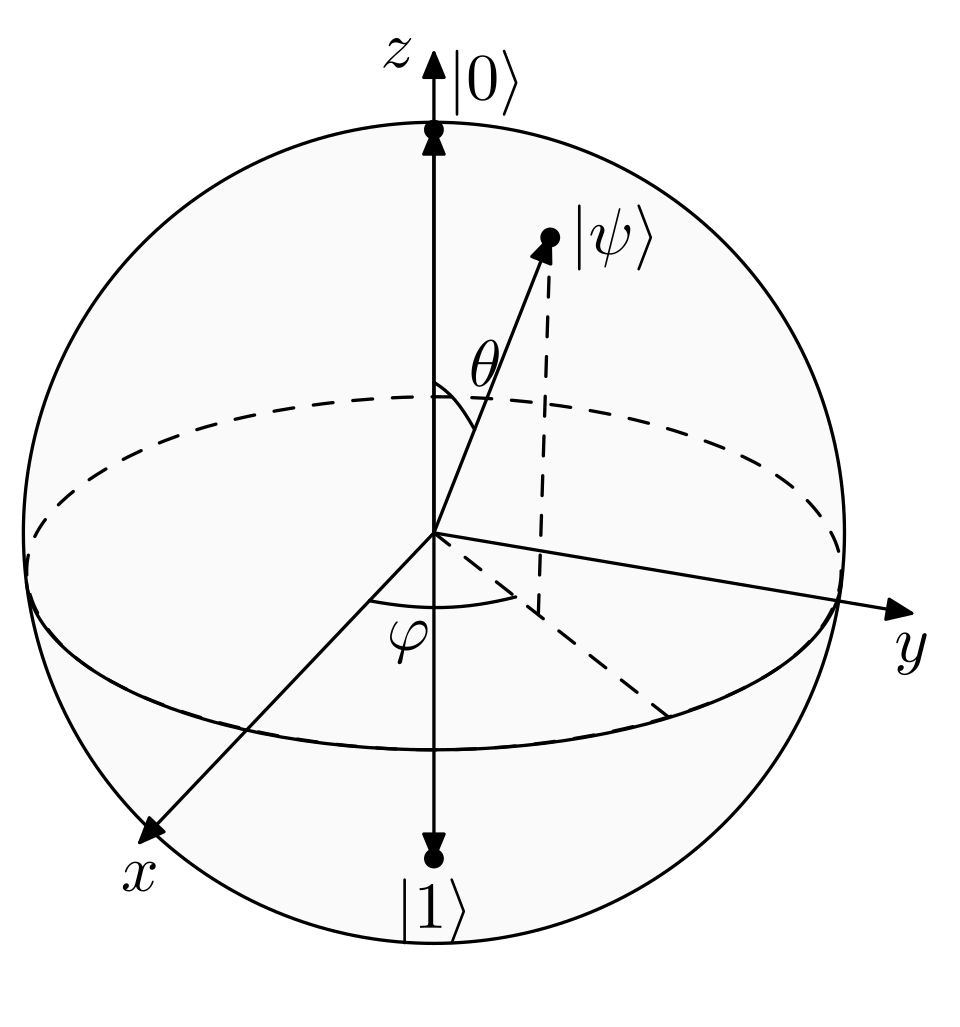
\includegraphics[scale=0.15]{Bloch_sphere.png}
\caption{Bloch sphere}
\end{figure}
\end{frame}

\begin{frame}{Postulates of quantum mechanics}
\justify
\textbf{Postulate 4:} The state space of a composite physical system is the tensor product of the state spaces of the component physical systems. Moreover, if we have systems numbered 1 through $n$, and system number $i$ is prepared in the state $|\psi_i\rangle$, then the joint state of the total system is
\begin{align}
|\psi_1\rangle \otimes |\psi_2\rangle \otimes \ldots \otimes |\psi_n\rangle.
\end{align}
\vfill
Postulate 4 enables us to define quantum entanglement. Suppose we are given two qubit states, $|\psi\rangle \in \mathcal{H}_A = \mathbb{C}^2$ and $|\phi\rangle \in \mathcal{H}_B = \mathbb{C}^2$. The two-qubit state $|\psi_{AB}\rangle$ is entangled if $|\psi_{AB}\rangle \neq |\psi\rangle \otimes |\phi\rangle$.
\vfill
For example, the following state $|\psi_{AB}\rangle$ is separable,
\begin{align*}
|\psi_{AB}\rangle & = \frac{1}{2} (|00\rangle + |01\rangle + |10\rangle + |11\rangle) \\
& = \frac{1}{2} [|0\rangle \otimes (|0\rangle + |1\rangle) + |1\rangle \otimes (|0\rangle + |1\rangle)] \\
& = \frac{1}{2} (|0\rangle + |1\rangle) \otimes (|0\rangle + |1\rangle) \\
& = |+\rangle \otimes |+\rangle
\end{align*}
\end{frame}

\begin{frame}
\justify
It is not always obvious to identify if a given two-qubit state is separable or not. One can derive separability condition for two qubits. As long as the two-qubit state satisfies the separability condition, the two-qubit state is separable (else, it is entangled).
\vfill
Let $|\psi\rangle = \psi_0 |0\rangle + \psi_1 |1\rangle$, $|\phi\rangle = \phi_0 |0\rangle + \phi_1 |1\rangle$. Then
\begin{align*}
|\psi_{AB}\rangle & = |\psi\rangle \otimes |\phi\rangle \\
& = (\psi_0 |0\rangle + \psi_1 |1\rangle) \otimes (\phi_0 |0\rangle + \phi_1 |1\rangle) \\
& = \psi_0\phi_0 |00\rangle + \psi_0\phi_1 |01\rangle + \psi_1\phi_0 |10\rangle + \psi_1\phi_1 |11\rangle
\end{align*}
\vfill
Notice that the probability amplitudes of $|00\rangle$ and $|11\rangle$, when multiplied together, is the same as the product of probability amplitudes of $|10\rangle$ and $|01\rangle$. We can conclude that for a two-qubit state $|\psi_{AB}\rangle = \psi_{00}|00\rangle + \psi_{01}|01\rangle + \psi_{10}|10\rangle + \psi_{11}|11\rangle$, if $\psi_{00} \psi_{11} = \psi_{10} \psi_{01}$, the two-qubit state is separable. Else, it is entangled.
\end{frame}

\begin{frame}{Superdense coding}
\justify
Can Alice communicate a number of classical bits of information by transmitting a smaller number of qubits, under the assumption that Alice and Bob receive an entangled resource beforehand?
\vfill
\begin{itemize}
\item Alice and Bob initially share a pair of qubits in the Bell state,
\begin{align}
|\psi\rangle = \frac{|00\rangle + |11\rangle}{\sqrt{2}};
\end{align}
\item If Alice wants to send 00, she does nothing; If Alice wants to send 01, she applies $Z$; If Alice wants to send 10, she applies $X$; If Alice wants to send 11, she applies $iY$;
\end{itemize}
\end{frame}

\begin{frame}
\justify
\begin{itemize}
\item The final two-qubit state becomes:
\begin{align}
00: |\psi\rangle & \rightarrow \frac{|00\rangle + |11\rangle}{\sqrt{2}} \\
01: |\psi\rangle & \rightarrow \frac{|00\rangle - |11\rangle}{\sqrt{2}} \\
10: |\psi\rangle & \rightarrow \frac{|10\rangle + |01\rangle}{\sqrt{2}} \\
11: |\psi\rangle & \rightarrow \frac{|01\rangle - |10\rangle}{\sqrt{2}}
\end{align}
\item Alice sends her qubit to Bob;
\item Bob performs a Bell basis measurement to determine which of the four possible bit strings Alice sent.
\end{itemize}
\end{frame}

\begin{frame}
\justify
\begin{figure}[h!]
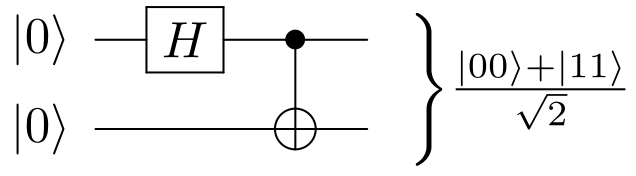
\includegraphics[scale=0.3]{Bell_basis.png}
\caption{Bell state creation}
\end{figure}
\vfill
\begin{figure}[h!]
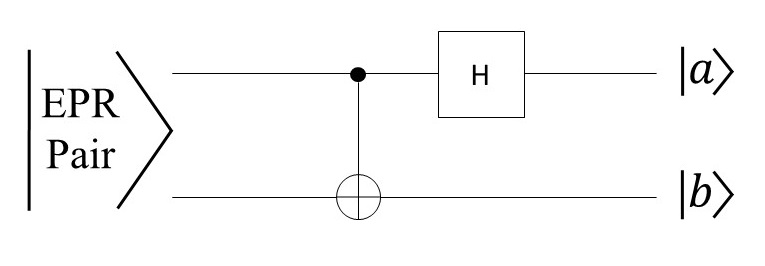
\includegraphics[scale=0.3]{Bell_basis_decoder.jpg}
\caption{Bell basis measurement}
\end{figure}
\end{frame}

\section{QMS Journal Club 4th meeting}
\begin{frame}
\vfill
\centering
\begin{beamercolorbox}[sep=8pt,center,shadow=true,rounded=true]{title}
\Large QMS Journal Club 4th meeting
\end{beamercolorbox}
\vfill
\end{frame}

\begin{frame}{Polarization vectors and density matrix}
\justify
Consider a vertically polarized photon, given by
\begin{align}
|V\rangle = \frac{|L\rangle + |R\rangle}{\sqrt{2}}.
\end{align}
\vfill
When the photon passes through a circular polarizer that allows either only $|L\rangle$ or only $|R\rangle$ polarized light, half of the photons will be absorbed in both cases.
\vfill
This may seem like half of the photons are in $|L\rangle$ or $|R\rangle$, but this is not true.
\vfill
If the photon passes through a linear polarizer, there will be no absorption.
\vfill
Meanwhile, if we pass unpolarized light through any type of polarizer, half of the intensity of light will be lost.
\end{frame}

\begin{frame}
\justify
For the case of polarized light, the action of ``measuring" the polarization of light is contextual, i.e. the outcome depends on what kind of measurement is being performed.
\vfill
For the case of unpolarized light, the action of ``measuring" the polarization of light is not contextual, because the outcome does not depend on the type of measurement being performed.
\vfill
This suggests that for the case of polarized light, a quantum treatment is required (contextuality is a quantum phenomenon), whereas a classical treatment is required for the case of unpolarized light.
\vfill
Polarized light is one example of pure states, whereby the probability of obtaining $|L\rangle$ or $|R\rangle$ is given by the absolute square of the probability amplitude.
\end{frame}

\begin{frame}
\justify
Unpolarized light is one example of mixed states, and it is considered as a (classical) statistical ensemble, i.e. each photon having either $|R\rangle$ or $|L\rangle$ polarization with probability $\frac{1}{2}$.
\vfill
For this example,
\begin{align}
\rho = \frac{1}{2}|R\rangle \langle R| + \frac{1}{2}|L\rangle \langle L| = \frac{1}{2}|H\rangle \langle H| + \frac{1}{2}|V\rangle \langle V| = \frac{1}{2} \begin{pmatrix} 1 & 0 \\ 0 & 1 \end{pmatrix}.
\end{align}
\vfill
These two ensembles are completely indistinguishable experimentally, hence they are considered the same mixed state.
\vfill
Conventionally,
\begin{align}
|H\rangle & = |0\rangle,\, |V\rangle = |1\rangle, \\
|D\rangle & = |+\rangle,\, |A\rangle = |-\rangle, \\
|L\rangle & = |+i\rangle,\, |R\rangle = |-i\rangle.
\end{align}
\end{frame}

\begin{frame}
\justify
Formally, the density matrix of a quantum system is defined as
\begin{align}
\rho = \sum_i p_i |\psi_i\rangle \langle\psi_i|,
\end{align}
where $\sum_i p_i = 1$. We say that $\rho$ is a mixture of pure states.
\vfill
Density matrix is a more general formalism compared to state vector formalism, since a pure state $|\psi\rangle$ can be described by a density matrix $\rho = |\psi\rangle \langle\psi|$.
\vfill
Consider
\begin{align}
|\psi\rangle & = \psi_0|0\rangle + \psi_1|1\rangle, \\
|\phi\rangle & = \phi_0|0\rangle + \phi_1|1\rangle, \\
\rho & = p_\psi |\psi\rangle \langle\psi| + p_\phi |\phi\rangle \langle\phi|,
\end{align}
where $p_\psi + p_\phi = 1$. Find $\rho$ in a $2 \times 2$ matrix.
\end{frame}

\begin{frame}
\justify
The density matrix is given by
\begin{align}
\rho = \begin{pmatrix} p_\psi |\psi_0|^2 + p_\phi |\phi_0|^2 & p_\psi \psi_0 \bar{\psi}_1 + p_\phi \phi_0 \bar{\phi}_1 \\ p_\psi \bar{\psi}_0 \psi_1 + p_\phi \bar{\phi}_0 \phi_1 & p_\psi |\psi_1|^2 + p_\phi |\phi_1|^2 \end{pmatrix}.
\end{align}
If we compute $\langle 0 | \rho | 0 \rangle$, we get $p_\psi |\psi_0|^2 + p_\phi |\phi_0|^2$.
\vfill
The diagonal element gives the probability of finding a particle in the corresponding basis state $\{|0\rangle,\, |1\rangle\}$.
\vfill
For a general state $|\Psi\rangle$,
\begin{align}
\langle\Psi| \rho |\Psi\rangle & = p_\psi \langle\Psi|\psi\rangle \langle\psi|\Psi\rangle + p_\phi \langle\Psi|\phi\rangle \langle\phi|\Psi\rangle \nonumber \\
& = p_\psi |\langle\psi|\Psi\rangle|^2 + p_\phi |\langle\phi|\Psi\rangle|^2
\end{align}
it can be seen that $\langle\Psi| \rho |\Psi\rangle$ gives the total probability of finding a particle in the pure state $|\Psi\rangle$ within a mixture $\rho$.
\end{frame}

\begin{frame}
\justify
A density matrix $\rho$ has the following properties:
\begin{enumerate}
\item $Tr(\rho) = 1$;
\item $\rho^\dagger = \rho$;
\item It is a positive semi-definite matrix, i.e. $\langle\psi|\rho|\psi\rangle \geq 0$.
\end{enumerate}
\vfill
For pure states, the density matrix $\rho$ further satisfies the following:
\begin{enumerate}
\item $\rho^2 = \rho$;
\item $Tr(\rho^2) = 1$.
\end{enumerate}
\vfill
\textbf{Exercise:} How many real parameters do you need to describe a $2\times 2$ density matrix?
\end{frame}

\begin{frame}
\justify
You need three real parameters to describe a $2\times 2$ density matrix.
\vfill
Consider again the one-qubit state,
\begin{align}
|\psi\rangle = \cos\left(\frac{\theta}{2}\right) |0\rangle + e^{i \phi} \sin\left(\frac{\theta}{2}\right) |1\rangle.
\end{align}
\vfill
Its density matrix is given by
\begin{align}
\rho & = \begin{pmatrix}
\cos^2 \left(\frac{\theta}{2}\right) & e^{-i\phi} \sin \left(\frac{\theta}{2}\right) \cos \left(\frac{\theta}{2}\right) \\ e^{i\phi} \sin \left(\frac{\theta}{2}\right) \cos \left(\frac{\theta}{2}\right) & \sin^2 \left(\frac{\theta}{2}\right)
\end{pmatrix}
\end{align}
\vfill
Previously, we learn that
\begin{align}
P_x = \langle\psi|X|\psi\rangle & = \sin\theta \cos\phi, \\
P_y = \langle\psi|Y|\psi\rangle & = \sin\theta \sin\phi, \\
P_z = \langle\psi|Z|\psi\rangle & = \cos\theta.
\end{align}
\end{frame}

\begin{frame}
\justify
We want to rewrite the density matrix in terms of $\{P_x,\, P_y,\, P_z\}$, which are called the polarization (Bloch) vectors,
\begin{align}
\rho & = \begin{pmatrix}
\frac{\cos\theta +1}{2} & \frac{\sin\theta(\cos\phi - i \sin\phi)}{2} \\ \frac{\sin\theta (\cos\phi + i\sin\phi)}{2} & \frac{1-\cos\theta}{2}
\end{pmatrix} \nonumber \\
& = \frac{1}{2} \begin{pmatrix}
P_z + 1 & P_x - i P_y \\ P_x + iP_y & 1 - P_z
\end{pmatrix} \nonumber \\
& = \frac{1}{2} \left( I + P_x X + P_y Y + P_z Z \right) \nonumber \\
& = \frac{1}{2} \left( I + \vec{P} \cdot \vec{\sigma} \right),
\end{align}
where
\begin{align}
\vec{P} = \begin{pmatrix} P_x \\ P_y \\ P_z \end{pmatrix},\, \vec{\sigma} = \begin{pmatrix} X \\ Y \\ Z \end{pmatrix}.
\end{align}
\end{frame}

\begin{frame}
\justify
In general, a density matrix can be written as $\rho = \frac{1}{2} \left( I + \vec{r} \cdot \vec{\sigma} \right)$.
\vfill
Density matrix formalism is useful when
\begin{enumerate}
\item the preparation of a system can randomly produce different pure states, and thus one must deal with the statistics of the ensemble of possible preparations;
\item when one wants to describe a physical system that is entangled with another, without describing their combined state (i.e. finding the reduced density matrix of a subsystem).
\end{enumerate}
\end{frame}

\section{QMS Journal Club 5th meeting}
\begin{frame}
\vfill
\centering
\begin{beamercolorbox}[sep=8pt,center,shadow=true,rounded=true]{title}
\Large QMS Journal Club 5th meeting
\end{beamercolorbox}
\vfill
\end{frame}

\begin{frame}{Density matrix formalism}
\justify
Previously, we mentioned that density matrix formalism is useful when
\begin{enumerate}
\item the preparation of a system can randomly produce different pure states, and thus one must deal with the statistics of the ensemble of possible preparations;
\item when one wants to describe a physical system that is entangled with another, without describing their combined state (i.e. finding the reduced density matrix of a subsystem).
\end{enumerate}
\vfill
Consider the Bell state
\begin{align}
|\psi\rangle = \frac{|00\rangle + |11\rangle}{\sqrt{2}}.
\end{align}
\vfill
The description of this Bell state is that when measurement is performed for qubit $A$, there is a probability $\frac{1}{2}$ to get $|0\rangle$ or $|1\rangle$.
\vfill
How can we describe the quantum state for qubit $A$ alone?
\end{frame}

\begin{frame}
\justify
One might be tempted to write
\begin{align}
|\psi_A\rangle = \frac{1}{\sqrt{2}} (|0_A\rangle + |1_A\rangle).
\end{align}
\vfill
This description gives you the correct statistics when you measure in the Pauli $Z$ basis, but it gives you a wrong statistics when you measure in the Pauli $X$ basis because $|\psi_A\rangle$ is now its eigenstate, $|+\rangle$.
\vfill
This again shows that the state vector formalism does not completely capture the classical statistical ensemble aspect of mixed states.
\vfill
Previously, an example of maximally mixed state was given,
\begin{align}
\rho = \frac{1}{2}|R\rangle \langle R| + \frac{1}{2}|L\rangle \langle L| = \frac{1}{2}|H\rangle \langle H| + \frac{1}{2}|V\rangle \langle V| = \frac{1}{2} \begin{pmatrix} 1 & 0 \\ 0 & 1 \end{pmatrix}.
\end{align}
\vfill
Regardless of what measurement basis we are taking, we always get a probability of $\frac{1}{2}$ to get either $\{|R\rangle,\, |L\rangle\}$ (or $\{|H\rangle,\, |V\rangle\}$).
\end{frame}

\begin{frame}{Postulates of quantum mechanics}
\justify
\textbf{Postulate 1:} Associate to any isolated physical system is a complex vector space with inner product, known as the state space of the system. The system is completely described by its density operator, which is a positive semi-definite operator $\rho = \sum_i p_i |\psi_i\rangle \langle\psi_i|$ with trace one, acting on the state space of the system.
\vfill
\textbf{Postulate 2:} The evolution of a closed quantum system is described by a unitary transformation. The state $\rho$ of the system at time $t_1$ is related to the state $\rho'$ of the system at time $t_2$ by a unitary operator $U$,
\begin{align}
\rho' = U\rho U^\dagger.
\end{align}
\end{frame}

\begin{frame}
\justify
\textbf{Postulate 3:} Quantum measurements are described by a collection of measurement operators $M_m$, such that the probability that result $m$ occurs for the state of a quantum system $\rho$ is given by
\begin{align}
p(m) = Tr(M^\dagger_m M_m \rho),
\end{align}
and the state of the system after the measurement is
\begin{align}
\frac{M_m \rho M^\dagger_m}{Tr(M^\dagger_m M_m \rho)}.
\end{align}
\vfill
For projective measurement $M = \sum_m m |m\rangle \langle m|$ with projector $P_m = |m\rangle \langle m|$, $P_m^\dagger P_m = P_m$ and hence
\begin{align}
p(m) & = \sum_i p_i \langle\psi_i|P_m|\psi_i\rangle = \sum_i p_i \langle\psi_i|P_m \sum_j |j\rangle \langle j |\psi_i\rangle \nonumber \\
& = \sum_{ij} p_i \langle j |\psi_i\rangle \langle\psi_i|P_m |j\rangle = Tr \left(\sum_i p_i |\psi_i\rangle \langle\psi_i|P_m \right) \nonumber \\
& = Tr(\rho P_m) = Tr(P_m \rho).
\end{align}
\end{frame}

\begin{frame}
\justify
The expectation value of a measurement $M$ follows the same argument and can be written as
\begin{align}
\langle M \rangle = Tr(M \rho).
\end{align}
\vfill
\textbf{Postulate 4:} The state space of a composite quantum system is the tensor product of the state spaces of the component quantum systems, such that the joint state of the total system is $\rho_1 \otimes \rho_2 \otimes \ldots \otimes \rho_n$.
\vfill
Suppose that a density matrix is given as
\begin{align}
\rho = \frac{3}{4}|0\rangle \langle 0| + \frac{1}{4}|1\rangle \langle 1|.
\end{align}
\vfill
Let
\begin{align}
|a\rangle & = \sqrt{\frac{3}{4}} |0\rangle + \sqrt{\frac{1}{4}} |1\rangle, \\
|b\rangle & = \sqrt{\frac{3}{4}} |0\rangle - \sqrt{\frac{1}{4}} |1\rangle.
\end{align}
\end{frame}

\begin{frame}
\justify
Then,
\begin{align}
\rho = \frac{3}{4}|0\rangle \langle 0| + \frac{1}{4}|1\rangle \langle 1| = \frac{1}{2}|a\rangle \langle a| + \frac{1}{2}|b\rangle \langle b|.
\end{align}
\vfill
\textcolor[rgb]{1,0,0}{Different ensembles of quantum states can give rise to the same density matrix. When will two sets of state vectors $|\psi\rangle$ and $|\phi\rangle$ generate the same density matrix?}
\vfill
\textbf{\textcolor[rgb]{1,0,0}{Theorem:}} The sets $|\psi_i\rangle$ and $|\phi_j\rangle$ generate the same density matrix if and only if
\begin{align}
|\psi_i\rangle = \sum_j U_{ij} |\phi_j\rangle,
\end{align}
where $U_{ij}$ is a unitary matrix.
\end{frame}

\begin{frame}{Reduced density matrix}
\justify
Suppose we have a quantum system $A$ and $B$, defined by $\rho_{AB}$. The reduced density operator for system $A$ is defined by
\begin{align}
\rho_A = Tr_B(\rho_{AB}),
\end{align}
where $Tr_B$ is called partial trace over system $B$. Partial trace is defined by
\begin{align}
Tr_B (|a_1\rangle \langle a_2| \otimes |b_1\rangle \langle b_2|) = |a_1\rangle \langle a_2| Tr(|b_1\rangle \langle b_2|) = |a_1\rangle \langle a_2| \langle b_2 |b_1\rangle.
\end{align}
\vfill
\textbf{Exercise:} Consider the Bell state $|\psi_{AB}\rangle = \frac{|00\rangle + |11\rangle}{\sqrt{2}}$. Find the reduced density matrix of the second qubit.
\vfill
\textbf{Exercise:} Suppose a composite quantum system $A$ and $B$ is in the state $|a\rangle |b\rangle$. Show that the reduced density matrix of system $A$ is a pure state.
\end{frame}

\begin{frame}{Quantum teleportation}
\justify
Quantum teleportation begins with two parties, Alice and Bob, sharing a pair of entangled qubits in one of the Bell bases,
\begin{align}
\ket{\Phi}_{AB}^+ & = \frac{1}{\sqrt{2}} (\ket{00} + \ket{11}), \\
\ket{\Phi}_{AB}^- & = \frac{1}{\sqrt{2}} (\ket{00} - \ket{11}), \\
\ket{\Psi}_{AB}^+ & = \frac{1}{\sqrt{2}} (\ket{01} + \ket{10}), \\
\ket{\Psi}_{AB}^- & = \frac{1}{\sqrt{2}} (\ket{01} - \ket{10}).
\end{align}
Without loss of generality, we focus on the Bell basis $\ket{\Phi}_{AB}^+$ in our discussion. The other Bell bases follow the same mathematical arguments.
\end{frame}

\begin{frame}
\centering
\begin{figure}
\begin{quantikz}
\lstick{$\ket{\psi}_C$}   & \ctrl{1} & \gate{H} \slice{1} &             & \meter{M_C}    & \cwbend{2} \\
\lstick{$\ket{\Phi}_A^+$} & \targ{}  &                    & \meter{M_A} & \cwbend{1} \\
\lstick{$\ket{\Phi}_B^+$} &          &                    &             & \gate{X^{M_A}} & \gate{Z^{M_C}} \slice{2} & & \rstick{$\ket{\psi}_B$}
\end{quantikz}
\caption{Quantum teleportation}
\end{figure}
\end{frame}

\begin{frame}
\justify
Initially, the shared Bell state between Alice and Bob, and the qubit that Alice wants to send to Bob is given as:
\begin{align}
\ket{\psi}_{CAB} & = (\alpha \ket{0}_C + \beta \ket{1}_C) \otimes \frac{1}{\sqrt{2}} (\ket{00}_{AB} + \ket{11}_{AB}) \nonumber \\
& = \frac{1}{\sqrt{2}} (\alpha \ket{000} + \alpha \ket{011} + \beta \ket{100} + \beta \ket{111}).
\end{align}
After the CNOT gate, the above quantum state becomes:
\begin{align}
\ket{\psi}_{CAB} = \frac{1}{\sqrt{2}} (\alpha \ket{000} + \alpha \ket{011} + \beta \ket{110} + \beta \ket{101}).
\end{align}
\end{frame}

\begin{frame}
\justify
After the Hadamard gate, the quantum state at Step 1 will become:
\begin{align}
\ket{\psi}_{CAB} & = \frac{1}{\sqrt{2}} \left[ \frac{\alpha}{\sqrt{2}} (\ket{0}_C + \ket{1}_C) \otimes \ket{00}_{AB} + \frac{\alpha}{\sqrt{2}} (\ket{0}_C + \ket{1}_C) \otimes \ket{11}_{AB} \right. \nonumber \\ & \phantom{\frac{1}{\sqrt{2}}} \qquad \left. + \frac{\beta}{\sqrt{2}} (\ket{0}_C - \ket{1}_C) \otimes \ket{10}_{AB} + \frac{\beta}{\sqrt{2}} (\ket{0}_C - \ket{1}_C) \otimes \ket{01}_{AB} \right] \nonumber \\
& = \frac{1}{2} [ \alpha \ket{000} + \alpha \ket{100} + \alpha \ket{011} + \alpha \ket{111} + \beta \ket{010} - \beta \ket{110} \nonumber \\ & \qquad + \beta \ket{001} - \beta \ket{101}] \nonumber \\
& = \frac{1}{2} [ \ket{00}_{CA} (\alpha \ket{0}_B + \beta \ket{1}_B) + \ket{01}_{CA} (\beta \ket{0}_B + \alpha \ket{1}_B) \nonumber \\ & \qquad + \ket{10}_{CA} (\alpha \ket{0}_B - \beta \ket{1}_B) + \ket{11}_{CA} ( -\beta \ket{0}_B + \alpha \ket{1}_B)].
\end{align}
\end{frame}

\begin{frame}
\justify
In Step 2, quantum measurements will be performed on Alice's qubits (qubit $A$ and $C$) and the appropriate Pauli correction will be applied to Bob's qubit (qubit $B$) to recover the quantum information that is teleported. In short,
\begin{enumerate}
\item If the quantum measurement results in $\ket{00}_{CA}$, nothing ($\sigma_0 = \left( \begin{smallmatrix} 1 & 0 \\ 0 & 1 \end{smallmatrix} \right)$) will be performed;
\item If the quantum measurement results in $\ket{01}_{CA}$, Pauli $X$, $\sigma_1 = \left( \begin{smallmatrix} 0 & 1 \\ 1 & 0 \end{smallmatrix} \right)$ will be performed;
\item If the quantum measurement results in $\ket{10}_{CA}$, Pauli $Z$, $\sigma_3 = \left( \begin{smallmatrix} 1 & 0 \\ 0 & -1 \end{smallmatrix} \right)$ will be performed;
\item If the quantum measurement results in $\ket{11}_{CA}$, Pauli $Y$ up to a global phase of $i$, $i \sigma_2 = \left( \begin{smallmatrix} 0 & 1 \\ -1 & 0 \end{smallmatrix} \right)$ will be performed.
\end{enumerate}
\end{frame}

\begin{frame}
\justify
Find the density matrix of $|\psi\rangle_{CAB}$,
\begin{align}
|\psi\rangle_{CAB} & = \frac{1}{2} [ \ket{00} (\alpha \ket{0} + \beta \ket{1}) + \ket{01} (\beta \ket{0} + \alpha \ket{1}) \nonumber \\ & \qquad + \ket{10} (\alpha \ket{0} - \beta \ket{1}) + \ket{11} ( -\beta \ket{0} + \alpha \ket{1})].
\end{align}
Verify that when Alice's system is being traced out, the reduced density matrix of Bob is maximally mixed.
\vfill
This shows that any measurements performed by Bob will contain no information about $|\psi\rangle_{CAB}$, and Alice cannot use quantum teleportation to transmit information to Bob faster than speed of light.
\end{frame}

\begin{frame}
\justify
Here are some intermediate steps for your verifications. Let
\begin{align*}
|B_1\rangle & = \alpha \ket{0} + \beta \ket{1}, \\
|B_2\rangle & = \beta \ket{0} + \alpha \ket{1}, \\
|B_3\rangle & = \alpha \ket{0} - \beta \ket{1}, \\
|B_4\rangle & = -\beta \ket{0} + \alpha \ket{1}.
\end{align*}
\vfill
Then
\begin{align}
\rho_{AB} & = \frac{1}{4}[|0\rangle \langle 0| \otimes |B_1\rangle \langle B_1| + |0\rangle \langle 1| \otimes |B_1\rangle \langle B_2| + |1\rangle \langle 0| \otimes |B_2\rangle \langle B_1| \nonumber \\ & \qquad + |1\rangle \langle 1| \otimes |B_2\rangle \langle B_2| + |0\rangle \langle 0| \otimes |B_3\rangle \langle B_3| + |0\rangle \langle 1| \otimes |B_3\rangle \langle B_4| \nonumber \\ & \qquad + |1\rangle \langle 0| \otimes |B_4\rangle \langle B_3| + |1\rangle \langle 1| \otimes |B_4\rangle \langle B_4|].
\end{align}
\vfill
Lastly,
\begin{align}
\rho_B & = \frac{1}{4}[|B_1\rangle \langle B_1| + |B_2\rangle \langle B_2| + |B_3\rangle \langle B_3| + |B_4\rangle \langle B_4|] \nonumber \\
& = \frac{1}{4} [2(|\alpha|^2 + |\beta|^2) |0\rangle \langle 0| + 2(|\alpha|^2 + |\beta|^2) |1\rangle \langle 1|] = \frac{1}{2}I.
\end{align}
\end{frame}

\section{QMS Journal Club 6th meeting}
\begin{frame}
\vfill
\centering
\begin{beamercolorbox}[sep=8pt,center,shadow=true,rounded=true]{title}
\Large QMS Journal Club 6th meeting
\end{beamercolorbox}
\vfill
\end{frame}

\begin{frame}{Higher order tensors}
\justify
From one-qubit state
\begin{align}
|\psi_A\rangle = \psi_0 |0\rangle + \psi_1 |1\rangle
\end{align}
to two-qubit state
\begin{align}
|\psi_{AB}\rangle = \psi_{00} |00\rangle + \psi_{01} |01\rangle + \psi_{10} |10\rangle + \psi_{11} |11\rangle,
\end{align}
the probability amplitude of the quantum states changes from an one-index object to a two-index object.
\vfill
In general, one-index object $\Psi_A = (\psi_i)$ is called tensor of order 1, while two-index object $\Psi_{AB} = (\psi_{ij})$ is called tensor of order 2.
\vfill
Tensor of order 1 is usually represented as a column vector and it coincides with the state vector representation.
\vfill
Meanwhile, tensor of order 2 is represented as a matrix. In two-qubit case,
\begin{align}
\Psi_{AB} = (\psi_{ij}) = \begin{pmatrix}
\psi_{00} & \psi_{01} \\ \psi_{10} & \psi_{11}
\end{pmatrix}.
\end{align}
\end{frame}

\begin{frame}{Schmidt decomposition}
\justify
Theorem: Suppose $|\psi\rangle$ is a pure state of a composite system $AB$. Then there exist orthonormal states $|i_A\rangle$ for system $A$, and orthonormal states $|i_B\rangle$ for system $B$, such that
\begin{align}
|\psi\rangle = \sum_i \lambda_i |i_A\rangle |i_B\rangle,
\end{align}
where $\lambda_i$ are non-negative real numbers satisfying $\sum_i \lambda_i^2 = 1$, known as Schmidt coefficients.
\vfill
Schmidt decomposition is a consequence of singular value decomposition when representing $|\psi\rangle$ as a tensor of order 2,
\begin{align}
\Psi_{AB} = U \Lambda V^T,
\end{align}
where $U$ and $V$ are unitary matrices and $\Lambda$ is a diagonal matrix.
\end{frame}

\begin{frame}
\justify
Singular value decomposition works for rectangular matrices. As a consequence of this, Schmidt decomposition works for any bipartite quantum systems of different dimension, for example qubit-qutrit system.
\vfill
As a convention, we usually require an ordering condition, i.e. $\lambda_1 \geq \lambda_2 \geq \ldots \geq \lambda_n$. This makes sure that the unitary matrices $U$ and $V$ to be uniquely determined.
\vfill
For two qubits, the reduced density matrices $\rho_A$ and $\rho_B$ are
\begin{align}
\rho_A & = \begin{pmatrix} |\psi_{00}|^2 + |\psi_{01}|^2 & \psi_{00} \bar{\psi}_{10} + \psi_{01} \bar{\psi}_{11} \\ \bar{\psi}_{00} \psi_{10} + \bar{\psi}_{01} \psi_{11} & |\psi_{10}|^2 + |\psi_{11}|^2 \end{pmatrix}, \\
\rho_B & = \begin{pmatrix} |\psi_{00}|^2 + |\psi_{10}|^2 & \psi_{00} \bar{\psi}_{01} + \psi_{10} \bar{\psi}_{11} \\ \bar{\psi}_{00} \psi_{01} + \bar{\psi}_{10} \psi_{11} & |\psi_{01}|^2 + |\psi_{11}|^2 \end{pmatrix}.
\end{align}
\vfill
\textbf{Exercise:} Show that
\begin{align}
\rho_A & = \Psi_{AB} \Psi_{AB}^\dagger, \\
\rho_B & = \Psi_{AB}^T \bar{\Psi}_{AB}.
\end{align}
\end{frame}

\begin{frame}
\justify
As a result, when singular value decomposition is applied,
\begin{align}
\rho_A & = \Psi_{AB} \Psi_{AB}^\dagger = U \Lambda V^T \bar{V} \Lambda U^\dagger = U \Lambda^2 U^\dagger, \\
\rho_B & = \Psi_{AB}^T \bar{\Psi}_{AB} = V \Lambda U^T \bar{U} \Lambda V^\dagger = V \Lambda^2 V^\dagger.
\end{align}
\vfill
This shows that $U$ and $V$ are the eigendecomposition of the reduced density matrices $\rho_A$ and $\rho_B$ respectively, and the reduced density matrices $\rho_A$ and $\rho_B$ have the same eigenvalues (singular values or Schmidt coefficients).
\vfill
For two qubits, there are two Schmidt coefficients $\lambda_1$ and $\lambda_2$, and we know that $\lambda_1^2 + \lambda_2^2 = 1$. Therefore, there are only three possibilities,
\begin{enumerate}
\item Maximally entangled states: $\lambda_1^2 = \lambda_2^2 = \frac{1}{2}$
\item Entangled states: $\lambda_1^2 > \lambda_2^2 \neq 0$
\item Separable states: $\lambda_1^2 = 1,\, \lambda_2^2 = 0$
\end{enumerate}
\end{frame}

\begin{frame}
\justify
\textbf{Exercise:} Classify the following two-qubit states according to the framework.
\begin{enumerate}
\item $\frac{1}{\sqrt{2}} (\ket{00} + \ket{11})$
\item $\frac{1}{\sqrt{3}} (\ket{00} + \ket{01} + \ket{10})$
\item $\frac{1}{2} (\ket{00} + \ket{01} + \ket{10} + \ket{11})$
\end{enumerate}
\vfill
One can also describe the separability of two-qubit states by finding the separability condition. Let $|\psi_A\rangle \in \mathcal{H}_A$ and $|\phi_B\rangle \in \mathcal{H}_B$, and
\begin{align}
|\psi_A\rangle & = \psi_0 |0\rangle + \psi_1 |1\rangle, \\
|\phi_B\rangle & = \phi_0 |0\rangle + \phi_1 |1\rangle.
\end{align}
\vfill
The combined two-qubit state becomes
\begin{align}
|\psi_{AB}\rangle & = |\psi_A\rangle \otimes |\phi_B\rangle \nonumber \\
& = \psi_0 \phi_0 |00\rangle + \psi_0 \phi_1 |01\rangle + \psi_1 \phi_0 |10\rangle + \psi_1 \phi_1 |11\rangle.
\end{align}
\end{frame}

\begin{frame}
\justify
One can notice that the product of probability amplitudes of $|00\rangle$ and $|11\rangle$ is the same as the product of probability amplitudes of $|01\rangle$ and $|10\rangle$, when the two-qubit state is separable.
\vfill
Therefore, the separability condition of two qubits is given by
\begin{align}
\psi_{00} \psi_{11} - \psi_{01} \psi_{10}.
\end{align}
\vfill
If $\psi_{00} \psi_{11} - \psi_{01} \psi_{10} = 0$, the two-qubit state is separable. Otherwise, it is entangled.
\vfill
Last but not least, notice that the separability condition of two qubits is the same as the determinant of $\Psi_{AB}$,
\begin{align}
\Psi_{AB} = (\psi_{ij}) = \begin{pmatrix}
\psi_{00} & \psi_{01} \\ \psi_{10} & \psi_{11}
\end{pmatrix}.
\end{align}
\vfill
The whole process is called entanglement classification of two qubits, which is well-studied for bipartite systems due to Schmidt decomposition.
\end{frame}

\begin{frame}
\justify
From group theoretic perspective, the action of $U$ and $V$ is called local unitary group action on two qubits. Notice that $U$ only acts on qubit $A$, $V$ only acts on qubit $B$. Hence, singular value decomposition (or equivalently, Schmidt decomposition) on a two-qubit state can be written as
\begin{align}
U \otimes V |\psi_{AB}\rangle & = \sum_{ij} U \otimes V \psi_{ij} |ij\rangle \nonumber \\
& = \sum_{ijklmn} \psi_{ij} |k\rangle \langle k| U |m\rangle \langle m| \otimes |l\rangle \langle l| V |n\rangle \langle n| (|i\rangle \otimes |j\rangle) \nonumber \\
& = \sum_{ijklmn} \psi_{ij} |k\rangle \langle k| U |m\rangle \langle m| i\rangle \otimes |l\rangle \langle l| V |n\rangle \langle n|j\rangle \nonumber \\
& = \sum_{ijkl} \psi_{ij} |k\rangle \langle k| U |i\rangle \otimes |l\rangle \langle l| V |j\rangle \nonumber \\
& = \sum_{ijkl} \psi_{ij} u_{ki} v_{lj} |k\rangle \otimes |l\rangle = \sum_{ijkl} u_{ki} \psi_{ij} v^T_{jl} |k\rangle \otimes |l\rangle
\end{align}
\vfill
\textbf{Exercise:} How many real parameters do you need to write down a $2 \times 2$ unitary matrix of determinant 1?
\end{frame}

\begin{frame}
\justify
You need 3 real parameters to define a $2 \times 2$ unitary matrix,
\begin{align}
U = \begin{pmatrix} u_{11} & u_{12} \\ -\bar{u}_{12} & \bar{u}_{11} \end{pmatrix}.
\end{align}
\vfill
In order to specify a generic two-qubit state, you need 6 real parameters (ignoring the global phase).
\vfill
Hence, it is possible for the local unitary group of two qubits to decompose a generic two-qubit state into the Schmidt coefficients, which are real and non-negative.
\vfill
\textbf{Exercise:} Can we have Schmidt decomposition for three qubits?
\end{frame}

\begin{frame}{State purification}
\justify
Suppose we are given a mixed state $\rho_A$. It is possible to introduce another (reference) system, $R$, in such a way that the combined quantum state $|AR\rangle$ is a pure state, and $\rho_A = Tr_R(|AR\rangle \langle AR|)$.
\vfill
Due to Schmidt decomposition, $\rho_A$ can be written as
\begin{align}
\rho_A = \sum_i p_i |i_A \rangle \langle i_A|.
\end{align}
\vfill
The combined system needs to be in this form
\begin{align}
|AR\rangle = \sum_i \sqrt{p_i} |i_A\rangle |i_R\rangle.
\end{align}
\vfill
The partial trace $Tr_R$ of the combined system is given by
\begin{align}
Tr_R(|AR\rangle \langle AR|) & = \sum_{ij} \sqrt{p_i p_j} |i_A\rangle \langle j_A| Tr(|i_R\rangle \langle j_R|) = \sum_{ij} \sqrt{p_i p_j} |i_A\rangle \langle j_A| \delta_{ij} \nonumber \\
& = \sum_i p_i |i_A\rangle \langle i_A| = \rho_A
\end{align}
\end{frame}

\section{QMS Journal Club 7th meeting}
\begin{frame}
\vfill
\centering
\begin{beamercolorbox}[sep=8pt,center,shadow=true,rounded=true]{title}
\Large QMS Journal Club 7th meeting
\end{beamercolorbox}
\vfill
\end{frame}

\begin{frame}{Quantum contextuality}
\justify
What is considered as ``physical"?
\vfill
Before quantum theory is developed, the intuition that we have is that the physical properties of an object exist independent of observation.
\vfill
Measurements merely act to reveal such physical properties.
\vfill
According to quantum theory, an unobserved particle does not possess physical properties that exist independent of observation.
\vfill
Such physical properties arise as a consequence of measurements performed upon the system.
\end{frame}

\begin{frame}
\justify
In order to counter this argument, one proposed the non-contextual hidden-variable theory, where
\begin{enumerate}
\item All quantum observables may be simultaneously assigned definite values, which may deterministically depend on some ``hidden" classical variable;
\item Value assignments pre-exist and are independent of the choice of any other observables;
\item Some functional constraints on the assignments of values for compatible observables are assumed.
\end{enumerate}
\vfill
Kochen and Specker proved that such hidden variable theory does not exist, i.e. it is impossible to assign definite values to an observable independent of other compatible observables (contexts).
\end{frame}

\begin{frame}
\justify
\begin{figure}[h!]
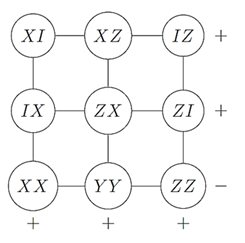
\includegraphics[scale=0.8]{Mermin-Peres_1.png}
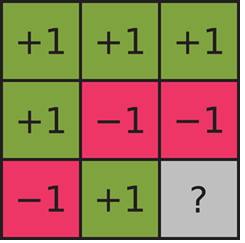
\includegraphics[scale=0.8]{Mermin-Peres_2.png}
\caption{Mermin-Peres square.}
\end{figure}
\vfill
Each line represents one context (mutually commuting operators) and each operator squares to identity, meaning that its eigenvalues are $\pm 1$.
\vfill
The product of the operators on each line is $I_1 I_2$, except for the last vertical context.
\vfill
There is no way to assign a definite value $\pm 1$ to each operator to reproduce these product rules because each operator appears in exactly two contexts.
\end{frame}

\begin{frame}{EPR paradox}
\justify
In a complete physical theory, there is an element corresponding to each element of reality. A sufficient condition for the reality of a physical quantity is \textbf{the possibility of predicting it with certainty, without disturbing the system}.
\vfill
In quantum mechanics, in the case of two physical quantities described by non-commuting operators, the knowledge of one precludes the knowledge of the other.
\vfill
Then, either
\begin{enumerate}
\item The description of reality given by the wavefunction in quantum mechanics is not complete;
\item These two quantities cannot have simultaneous reality.
\end{enumerate}
\end{frame}

\begin{frame}{Bell's theorem}
\justify
Bell's theorem assumes a local hidden variable model, whereby
\begin{enumerate}
\item ``local" refers to the principle of locality, i.e. an object is influenced directly only by its immediate surroundings. In order for a cause at one point to have an effect at another point, something in the space between those points must mediate the action.
\item ``Hidden variable" is a deterministic model to explain the probabilistic nature of quantum theory by introducing additional, possibly inaccessible, variables.
\end{enumerate}
\vfill
The correlations between the outcomes must obey a specific mathematical constraint, called Bell inequality.
\end{frame}

\begin{frame}
\justify
Consider the following setup:
\begin{enumerate}
\item Alice and Bob stand in widely separated locations. A pair of particles is prepared. One particle is sent to Alice, the other to Bob.
\item Alice and Bob are free to choose two possible measurements, $A_0$ and $A_1$, $B_0$ and $B_1$, respectively. Each of these measurements produce $\pm 1$.
\item Suppose that each measurement reveals a property that the particle already possessed. For example, if Alice chooses to measure $A_0$ and gets $+1$, then the particle she received has $+1$ for $a_0$.
\item Consider the combination for all possible properties $a_0,\, a_1,\, b_0,\, b_1$:
\begin{align}
a_0 b_0 + a_0 b_1 + a_1 b_0 - a_1 b_1 = (a_0 + a_1)b_0 + (a_0 - a_1)b_1.
\end{align}
\item Because $a_0$ and $a_1$ takes the values $\pm 1$, therefore it is either $a_0 = a_1$ or $a_0 = -a_1$. In the former case, $(a_0 - a_1)b_1 = 0$, while in the latter case, $(a_0 + a_1)b_0 = 0$. One of the terms on the RHS will vanish, and the remaining term will give $\pm 2$.
\item If the experiment repeats many times, the average will be given by
\begin{align}
|\langle A_0 B_0 \rangle + \langle A_0 B_1 \rangle + \langle A_1 B_0 \rangle - \langle A_1 B_1 \rangle| \leq 2.
\end{align}
\end{enumerate}
\end{frame}

\begin{frame}
\justify
Quantum entanglement violates this formulation of Bell inequality, called Clauser-Horne-Shimony-Holt (CHSH) inequality.
\vfill
Consider the bell state,
\begin{align}
|\psi\rangle = \frac{|01\rangle - |10\rangle}{\sqrt{2}}.
\end{align}
\vfill
The first qubit is passed to Alice, while the second to Bob. Alice and Bob measure the following observables,
\begin{align*}
A_0 = \sigma_z,\, A_1 = \sigma_x;\, B_0 = -\frac{\sigma_x + \sigma_z}{\sqrt{2}},\, B_1 = \frac{\sigma_x - \sigma_z}{\sqrt{2}}.
\end{align*}
\vfill
The expectation values are
\begin{align*}
\langle A_0 \otimes B_0 \rangle = \langle A_0 \otimes B_1 \rangle = \langle A_1 \otimes B_0 \rangle = \frac{1}{\sqrt{2}},\, \langle A_1 \otimes B_1 \rangle = - \frac{1}{\sqrt{2}}.
\end{align*}
\vfill
Therefore, the CHSH inequality is violated,
\begin{align}
\langle A_0 B_0 \rangle + \langle A_0 B_1 \rangle + \langle A_1 B_0 \rangle - \langle A_1 B_1 \rangle = 2\sqrt{2}.
\end{align}
\end{frame}

\begin{frame}{Quantum resource theory}
\justify
In studying algorithms, three questions concern us:
\begin{enumerate}
\item What resources are required to perform a given computational task?
\item What computational tasks are possible?
\item What are the limitations (lower bounds) of the number of operations that must be performed by any algorithm?
\end{enumerate}
\vfill
Quantum resource theory studies quantum information processes under a restricted set of physical operations.
\vfill
The permissible operations are ``free". Since they do not encompass all physical processes, only certain physically realizable states can be prepared. These accessible states are ``free".
\vfill
The ``prohibited" operations create ``resource" states.
\vfill
In quantum computing, entanglement is considered as a resource. The ``free" operations are local quantum operation and classical communication (LOCC). Entanglement cannot be generated by LOCC.
\end{frame}

\section{QMS Journal Club 8th meeting}
\begin{frame}
\vfill
\centering
\begin{beamercolorbox}[sep=8pt,center,shadow=true,rounded=true]{title}
\Large QMS Journal Club 8th meeting
\end{beamercolorbox}
\vfill
\end{frame}

\begin{frame}{Turing machines}
\justify
A Turing machine is an idealized computer with a simpler set of basic instructions and an idealized unbounded memory.
\vfill
We are addressing the second question: What computational tasks are possible?
\vfill
Hilbert's \textit{Entscheidungsproblem}, or the decision problem, asks whether or not there exists some algorithm which could be used to solve all the problems of mathematics.
\vfill
The answer to this is no, proved by Church and Turing through Church-Turing thesis.
\end{frame}

\begin{frame}
\justify
A Turing machine contains four elements:
\begin{enumerate}
\item A program;
\item A finite state control, which acts like a microprocessor;
\item A tape, which acts like a computer memory;
\item A read-write tape-head, which points to the position on the tape.
\end{enumerate}
\vfill
\begin{figure}[h!]
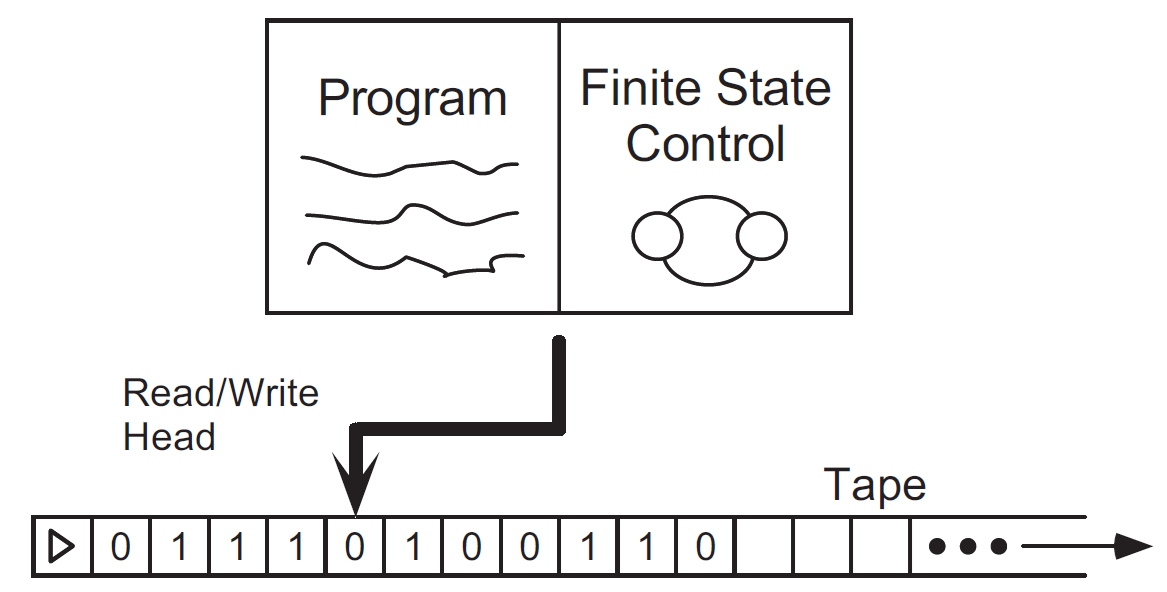
\includegraphics[scale=0.25]{Turing_machine.png}
\caption{A Turing machine.}
\end{figure}
\end{frame}

\begin{frame}
\justify
The finite state control consists of a finite set of internal states, $q_1,\,\ldots,\,q_m$.
\vfill
There are two special internal states, $q_s$ and $q_h$, referring to the starting state and halting state respectively.
\vfill
At the beginning of the computation, Turing machine is in the starting state $q_s$.
\vfill
If the computation finishes, the Turing machine ends up in the halting state $q_h$.
\vfill
The tape is a one-dimensional object which stretches off to infinity in one direction.
\vfill
The tape squares contain one symbol drawn from some alphabets $0,\,1,\,b,\,\triangleright$. $\triangleright$ marks the left edge of the tape.
\vfill
The tape-head identifies a single square on the tape as the square that is currently being accessed by the machine.
\end{frame}

\begin{frame}
\justify
A program for a Turing machine is a list of program lines of the form $\langle q,\,x,\,q',\,x',\,s \rangle$.
\vfill
$q$ is the state from the set of internal states of the Turing machine, while $x$ is the alphabet of symbols on the tape, $0,\,1,\,b,\,\triangleright$.
\vfill
Each cycle, the Turing machine looks through the program lines in order, searching for a line $\langle q,\,x,\,\cdot,\,\cdot,\,\cdot \rangle$, such that the current internal state is $q$ and the symbol being read is $x$.
\vfill
If the machine cannot find such a line, the internal state is changed to $q_h$, and the machine halts operation.
\vfill
If such a line is found, then the program line is executed.
\end{frame}

\begin{frame}
\justify
Execution of the program is as follows:
\begin{enumerate}
\item The internal state is changed to $q'$;
\item The symbol $x$ is overwritten by $x'$;
\item The tape-head moves left, right, or stands still, depending on whether $s$ is $-1,\,+1,\,0$ respectively. The only exception is if the tape-head is at the leftmost square and $s=-1$, then the tape-head stays put.
\end{enumerate}
\vfill
\textbf{Exercise:} Let $T$ be a Turing machine defined by the five tuples:
\begin{align*}
& \langle q_s,\,\triangleright,\,q_1,\,\triangleright,\,+1 \rangle,\, \langle q_1,\,0,\,q_1,\,b,\,+1 \rangle,\, \langle q_1,\,1,\,q_1,\,b,\,+1 \rangle,\, \langle q_1,\,b,\,q_2,\,b,\,-1 \rangle,\\ & \langle q_2,\,b,\,q_2,\,b,\,-1 \rangle,\, \langle q_2,\,\triangleright,\,q_3,\,\triangleright,\,+1 \rangle,\, \langle q_3,\,b,\,q_h,\,1,\,0 \rangle
\end{align*}
For each of these initial tapes, determine the final tape when $T$ halts.
\begin{enumerate}
\item $\triangleright,\, 0,\, 0,\, 1,\, 1,\, b$
\item $\triangleright,\, 1,\, 0,\, 1,\, 0,\, b$
\end{enumerate}
What is this Turing machine trying to compute?
\end{frame}

\begin{frame}
\justify
\textbf{Exercise:} Let $T$ be the Turing machine defined by the five-tuples:
\begin{align*}
& \langle q_0,\,0,\,q_1,\,1,\,+1 \rangle,\, \langle q_0,\,1,\,q_1,\,0,\,+1 \rangle,\, \langle q_0,\,b,\,q_1,\,0,\,+1 \rangle,\, \langle q_1,\,0,\,q_2,\,1,\,-1 \rangle,\\ & \langle q_1,\,1,\,q_1,\,0,\,+1 \rangle,\, \langle q_1,\,b,\,q_2,\,0,\,-1 \rangle
\end{align*}
For each of these initial tapes, determine the final tape when $T$ halts.
\begin{enumerate}
\item $0,\,0,\,1,\,1,\,b,\,b$
\item $1,\,0,\,1,\,b,\,b,\,b$
\item $b,\,b,\,b,\,b,\,b,\,b$
\end{enumerate}
\vfill
\textbf{Exercise:} What does the Turing machine described by the five-tuples
\begin{align*}
& \langle q_0,\,0,\,q_0,\,0,\,+1 \rangle,\, \langle q_0,\,1,\,q_1,\,0,\,+1 \rangle,\, \langle q_0,\,b,\,q_2,\,b,\,+1 \rangle,\, \langle q_1,\,0,\,q_1,\,0,\,+1 \rangle,\\ & \langle q_1,\,1,\,q_0,\,1,\,+1 \rangle,\, \langle q_1,\,b,\,q_2,\,b,\,+1 \rangle
\end{align*}
do when given the following tapes as input?
\begin{enumerate}
\item $1,\,1,\,b,\,b,\,b,\,b,\,b,\,b$
\item an arbitrary bit string
\end{enumerate}
\end{frame}

\begin{frame}
\justify
\textbf{Exercise:} Construct a Turing machine with tape symbols $0,\,1,\,b$ that, when given a bit string as input, replaces the first $0$ with a $1$ and does not change any of the other symbols on the tape.
\vfill
\textbf{Exercise:} Construct a Turing machine that recognizes the set of all bit strings that contain an even number of $1$s.
\vfill
\textbf{Exercise:} Describe a Turing machine to add two binary numbers $x$ and $y$ modulo 2. The numbers are input on the Turing machine tape in binary, in the form $x$, followed by a single blank, followed by $y$. If one number is not as long as the other, then you may assume that it has been padded with leading 0s to make the two numbers the same length.
\end{frame}

\begin{frame}
\justify
The initial state of the tape is used to represent the input to the function, and the final state of the tape is used to represent the output of the function.
\vfill
The Turing machine completely captures the notion of computing a function using an algorithm.
\vfill
\textbf{Church-Turing thesis:} The class of functions computable by a Turing machine corresponds exactly to the class of functions which we would naturally regards as being computable by an algorithm.
\vfill
Quantum computer also obey the Church-Turing thesis. The difference is the efficiency with which the computation of the function may be performed. Some functions can be computed much more efficiently on a quantum computer.
\vfill
There are different types of Turing machines. They are equivalent in the sense that each model is able to simulate the other. A universal Turing machine is a Turing machine that can simulate all other Turing machines and hence any possible computation.
\end{frame}

\begin{frame}{The Halting problem}
\justify
The Halting problem asks if the Turing machine with number $x$ halt upon input of the number $y$, i.e. if the algorithm halts or not.
\vfill
Turing defined the halting function,
\begin{align}
h(x) = \begin{cases}
0 & \text{if machine number $x$ does not halt upon input of $x$} \\
1 & \text{if machine number $x$ halts upon input of $x$}
\end{cases}
\end{align}
\vfill
If there is an algorithm to solve the halting problem, then there is an algorithm to evaluate $h(x)$. Consider the algorithm\newline
\texttt{$y=h(x)$\newline
if $y=0$ then halt\newline
else loop forever\newline
end if}
\vfill
This causes a contradiction. Therefore, the initial assumption that there is an algorithm to evaluate $h(x)$ must have been wrong.
\end{frame}

\section{QMS Journal Club 9th meeting}
\begin{frame}
\vfill
\centering
\begin{beamercolorbox}[sep=8pt,center,shadow=true,rounded=true]{title}
\Large QMS Journal Club 9th meeting
\end{beamercolorbox}
\vfill
\end{frame}

\begin{frame}{Circuit model of computation}
\justify
An alternative computational model is by using circuit.
\vfill
A circuit is made up of wires and logic gates.
\vfill
A logic gate is a function $f:\{0,\,1\}^k \rightarrow \{0,\,1\}^l$ from some fixed number $k$ of input bits to some fixed number $l$ of output bits.
\vfill
No loops are allowed in the circuit to avoid possible instabilities.
\vfill
Some important logic gates are:
\begin{enumerate}
\item FANOUT gate: Replace a bit with two copies of itself
\item CROSSOVER gate: The value of two bits are interchanged
\item AND gate
\item OR gate
\item NOT gate
\item NAND gate
\item NOR gate
\end{enumerate}
\vfill
Additionally, one allows the preparation of ancilla bits to allow extra working space during the computation.
\end{frame}

\begin{frame}
\justify
A few logic gates can be used to compute any function $f:\{0,\,1\}^k \rightarrow \{0,\,1\}^l$.
\vfill
The proof is by induction, starting from the simplest case, called the Boolean function $f:\{0,\,1\}^n \rightarrow \{0,\,1\}$.
\vfill
There are four possible functions:
\begin{enumerate}
\item Identity: Wire
\item Bit flip: NOT gate
\item Constant function $f(x) = 0$: AND with ancilla 0 bit
\item Constant function $f(x) = 1$: OR with ancilla 1 bit
\end{enumerate}
\vfill
The induction follows by increasing the number of bits through cascading the circuits and logic gates from the above.
\end{frame}

\begin{frame}
\justify
The set of such logic gates is called the (complete) universal logic set.
\vfill
Examples of universal logic set are
\begin{enumerate}
\item AND, OR and NOT
\item AND and NOT
\item OR and NOT
\item NAND (minimal set)
\item NOR (minimal set)
\end{enumerate}
\vfill
\textbf{Exercise:} Show that the NAND gate can be used to simulate AND, XOR, and NOT gates, provided wires, ancilla bits and FANOUT are available.
\vfill
Not every classical logic gate can be implemented in a straightforward manner in quantum computing. Due to no-cloning theorem, FANOUT cannot be performed. AND and XOR gates are not invertible (quantum operations are unitary).
\end{frame}

\begin{frame}
\begin{figure}[h!]
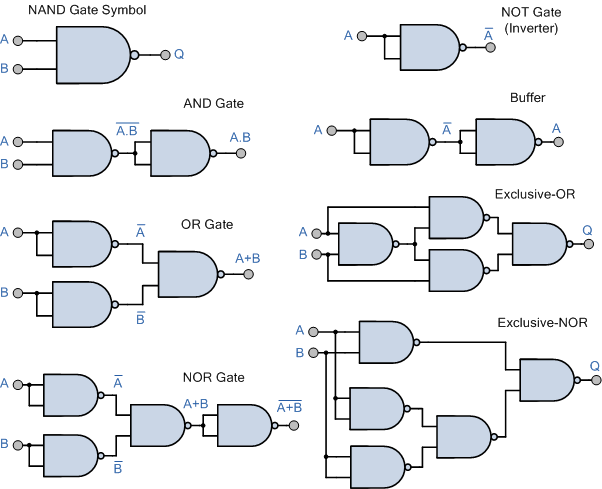
\includegraphics[scale=0.5]{NAND_universal.png}
\caption{NAND logic gate as the universal gate.}
\end{figure}
\end{frame}

\begin{frame}{Algorithm-based complexity}
\justify
Turing machine and the circuit model represent two different models of computation.
\vfill
On one hand, Turing machine is a uniform model, where the same computational device is used for all possible input lengths.
\vfill
On the other hand, the circuit model (Boolean circuit) is non-uniform, since inputs of different lengths are processed by different circuits.
\vfill
The concept of \textit{uniform circuit family} relates both models together by looking at the algorithm-based complexity.
\vfill
A circuit family consists of a collection of circuits $\{C_n\}$, where $C_n$ is a circuit with $n$ input bits.
\vfill
A circuit family is uniform if there is some algorithm running on a Turing machine which, upon input of $n$, generates a description of $C_n$.
\end{frame}

\begin{frame}
\justify
Different models of computation require different computational resources.
\vfill
One comparison is to look at the asymptotic behavior of a function, without worrying too much about the exact time count.
\vfill
For example, if a specific algorithm requires $24n+2\left\lceil \log n \right\rceil +16$ gates to perform, asymptotically the algorithm requires $n$ number of operations in the limit of large problem size.
\vfill
$O(g(n))$ is used to set the upper bounds $g(n)$ on the behavior of a function $f(n)$, i.e. for sufficiently large $n$, the function $g(n)$ is an upper bound on $f(n)$.
\vfill
$O(g(n))$ is useful for studying the worst-case behavior of specific algorithms.
\vfill
$\Omega(g(n))$ examines the lower bounds $g(n)$ on the behavior of a function $f(n)$, i.e. for sufficiently large $n$, $g(n)$ is a lower bound on $f(n)$.
\vfill
$\Theta(g(n))$ indicates that $f(n)$ behaves the same as $g(n)$ asymptotically. $f(n)$ is $\Theta(g(n))$ if it is both $O(g(n))$ and $\Omega(g(n))$.
\end{frame}

\begin{frame}
\justify
\textbf{Example:} $f(n)=2n$ is $O(n^2)$, since $2n \leq 2n^2$ for all positive $n$.
\vfill
\textbf{Example:} $f(n)=2^n$ is $\Omega(n^3)$, since $n^3 \leq 2^n$ for sufficiently large $n$.
\vfill
\textbf{Example:} $f(n)=7n^2 + \sqrt{n}\log n$ is $\Theta(n^2)$, since $7n^2 \leq f(x) \leq 8n^2$ for sufficiently large $n$.
\vfill
\textbf{\textcolor[rgb]{1,0,0}{Exercise:}} Show that $n^k$ is $O(n^{\log n})$ for any $k$, but that $n^{\log n}$ is never $O(n^k)$.
\vfill
\textbf{\textcolor[rgb]{1,0,0}{Exercise:}} Show that $c^n$ is $\Omega(n^{\log n})$ for any $c>1$, but that $n^{\log n}$ is never $\Omega(C^n)$.
\end{frame}

\begin{frame}
\justify
A simple compare-and-swap algorithm for solving the sorting problem is as follows.\\
\texttt{for j = 1 to n-1\\
\hspace{0.5cm} for k = j+1 to n\\
\hspace{1cm} compare-and-swap(j,k)\\
\hspace{0.5cm} end k\\
end j}
\vfill
This algorithm uses
\begin{align*}
(n-1) + (n-2) + \ldots + 1 = \frac{n(n-1)}{2}
\end{align*}
operations, hence it belongs to $\Theta(n^2)$.
\end{frame}

\begin{frame}{Computational complexity}
\justify
Computational complexity studies the lower bounds on the resources required by the best possible algorithm for solving a problem, even if the algorithm is not explicitly known.
\vfill
Ideally, the most efficient algorithm would match with the lower bound proved by computational complexity, but this is often not the case.
\vfill
A coarse classification of computational problems is to ask whether or not a problem can be solved using resources bounded by a polynomial in $n$ (\textbf{P}), or exponential (\textbf{NP}).
\vfill
A problem is regarded as \textit{easy, tractable, or feasible} if an algorithm for solving the problem using polynomial resources exists. Otherwise, it is \textit{hard, intractable, or infeasible}.
\vfill
\textbf{P} and \textbf{NP} are theoretical constructs. In reality, an algorithm using more operations is probably more useful than an optimized and efficient algorithm.
\end{frame}

\begin{frame}
\justify
\textbf{Strong Church-Turing thesis:} Any model of computation can be simulated on a probabilistic Turing machine with at most a polynomial increase in the number of elementary operations required.
\vfill
A probabilistic Turing machine is a non-deterministic Turing machine that chooses between the available transitions at each point according to some probability distribution. It was observed to be the strongest reasonable model of computation.
\vfill
In other words, if a problem has no polynomial resource solution on a probabilistic Turing machine, then it has no efficient solution on any computing device.
\end{frame}

\section{QMS Journal Club 10th meeting}
\begin{frame}
\vfill
\centering
\begin{beamercolorbox}[sep=8pt,center,shadow=true,rounded=true]{title}
\Large QMS Journal Club 10th meeting
\end{beamercolorbox}
\vfill
\end{frame}

\begin{frame}{Complexity classes}
\justify
Many computational problems can be framed as decision problems, primarily because the problems take their simplest form for analysis, but generalizable to other complex scenarios.
\vfill
A language $L$ over the alphabet $\sum$ is a subset of the set $\sum^*$ of all (finite) strings of symbols from $\sum$.
\vfill
\textbf{Example:} To convert the primarity decision problem into formal language, the binary alphabet is $\sum = \{0,\,1\}$. $\sum^*$ can be interpreted as non-negative integers. $L$ is defined to consist of all prime numbers in binary strings.
\vfill
Turing machine can be ``tuned" to have two halting states, $q_Y$ and $q_N$, to represent `yes' and `no' respectively.
\vfill
A language $L$ is decided by a Turing machine if the machine is able to decide whether an input $x$ on its tape is a member of the language of $L$ or not, eventually halting in the state $q_Y$ if $x \in L$, and $q_N$ if $x \notin L$.
\end{frame}

\begin{frame}
\justify
A problem is in \textbf{TIME}$(f(x))$ if there exists a Turing machine which decides whether a candidate $x$ is in the language in time $O(f(n))$, where $n$ is the length of $x$.
\vfill
Previously, we mentioned a coarse classification of computational problems by looking at the computational resources, either bounded by a polynomial in $n$ (\textbf{P}) or exponential (\textbf{NP}).
\vfill
An \textbf{NP} problem is that the `yes' instances of a problem can be easily verified with the aid of an appropriate \textit{witness}, while there is no need to produce a witness to $x \notin L$.
\vfill
The asymmetry of \textbf{NP} prompted a new class of languages, \textbf{coNP} which have witnesses to `no' instances.
\end{frame}

\begin{frame}
\justify
\begin{figure}[h!]
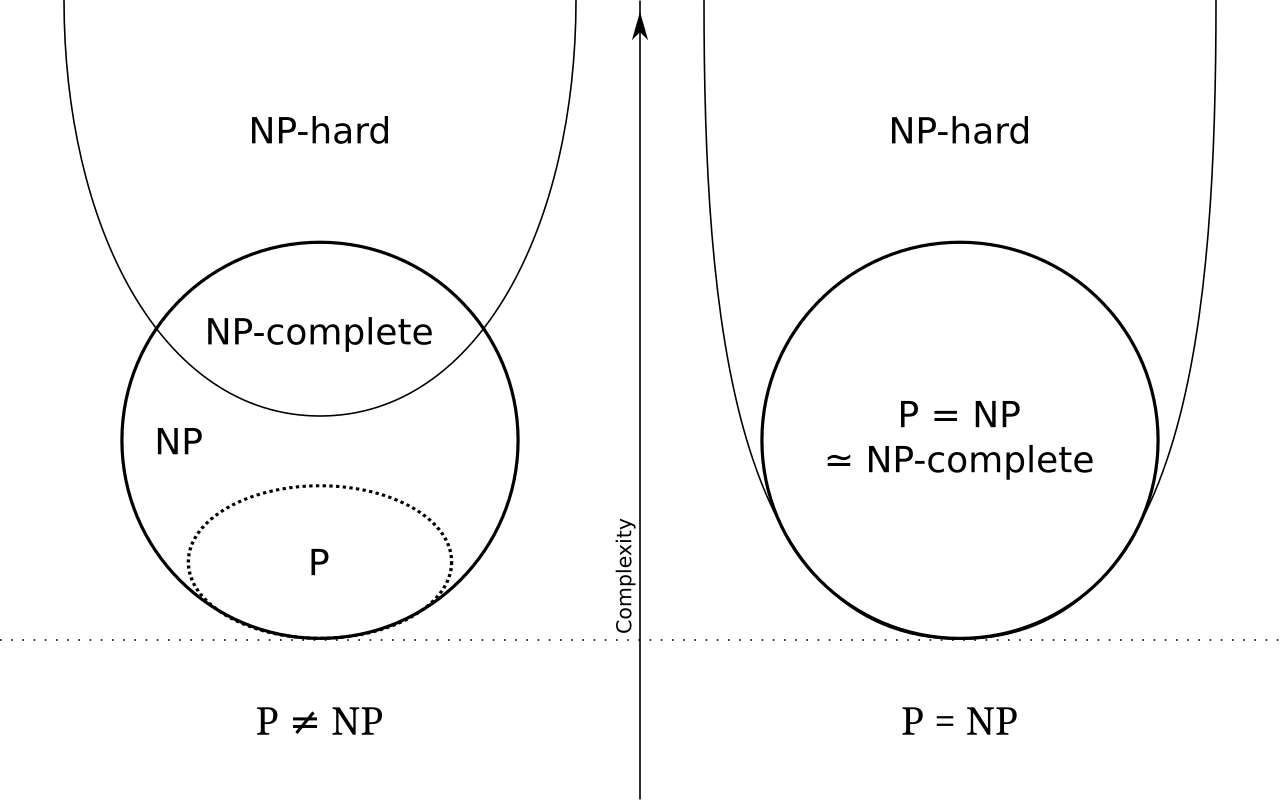
\includegraphics[scale=0.25]{p_vs_np.png}
\caption{\textbf{P} $\neq$ \textbf{NP} problem}
\end{figure}
\end{frame}

\begin{frame}{Hamiltonian vs Euler cycle problem}
\justify
A cycle is a sequence of vertices, $v_1,\,\ldots,\, v_m$ such that each pair of vertices $(v_j,\,v_{j+1})$ defines an edge.
\vfill
A simple cycle is a cycle in which none of the vertices is repeated, except for the first and last vertices.
\vfill
A Hamiltonian cycle is a simple cycle which visits every vertex in the graph.
\begin{figure}[h!]
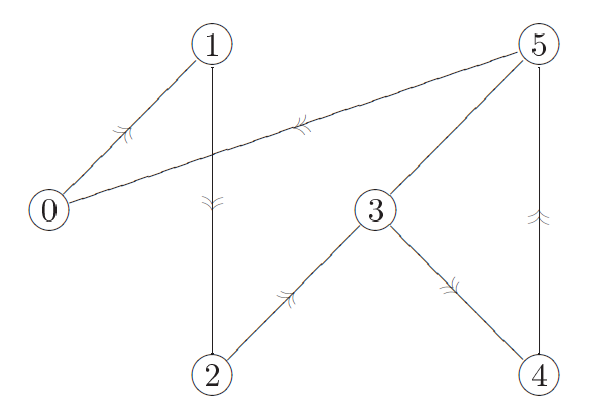
\includegraphics[scale=0.3]{Hamiltonian_cycle.png}
\caption{A Hamiltonian cycle}
\end{figure}
\end{frame}

\begin{frame}
\justify
The Hamiltonian cycle problem determines whether a given graph contains a Hamiltonian cycle or not.
\vfill
It is a problem in the class of \textbf{NP}-complete problems. Any other \textbf{NP} problems can be reduced to \textbf{NP}-complete problems in polynomial time, and that the solution is verifiable in polynomial time.
\vfill
If any \textbf{NP}-complete problem has a polynomial time solution, then \textbf{P} $=$ \textbf{NP}.
\vfill
The Hamiltonian cycle problem can be reduced to the traveling salesman problem, which asks that given a list of cities and the distances between each pair of cities, what is the shortest possible route that visits each city exactly once and returns to the origin city?
\vfill
Suppose we have a graph of $n$ vertices. By defining $d_{ij} = 1$ if vertices $i$ and $j$ are connected, and $d_{ij} = 2$ if vertices $i$ and $j$ are not connected, we convert the traveling salesman problem into the Hamiltonian cycle problem by finding the distance $d = n+1$. If a tour is of distance $d = n$, then it is a Hamiltonian cycle. Conversely is true.
\end{frame}

\begin{frame}
\justify
A language $B$ is said to be reducible to another language $A$ if there exists a Turing machine operating in polynomial time such that given input $x$ and output $R(x)$, $x \in B$ if and only if $R(x) \in A$.
\vfill
It means that if we have an algorithm for deciding $A$, then with a little extra overhead we can decide the language $B$.
\vfill
There is a language $L$ in the complexity class which is the ``most difficult" to decide, in the sense that every other language in the complexity class can be reduced to $L$. This is called a \textit{complete} problem.
\end{frame}

\begin{frame}
\justify
An Euler cycle is an ordering of the edges of a graph $G$ so that every edge in the graph is visited exactly once.
\vfill
The Euler cycle problem determines whether a given graph contains a Euler cycle or not.
\vfill
The Euler cycle problem is exactly the same problem as the Hamiltonian cycle problem, the only difference being that vertices are changed to edges.
\vfill
\textbf{Theorem:} A connected graph contains an Euler cycle if and only if every vertex has an even number of edges incident upon it.
\vfill
The theorem above provides a method to efficiently solve the Euler cycle problem, and thus the Euler cycle problem is in \textbf{P}.
\end{frame}

\begin{frame}
\justify
Assuming \textbf{P} $\neq$ \textbf{NP}, another class of problems called \textbf{NPI}, which is neither solvable with polynomial resources nor \textbf{NP}-complete is proposed.
\vfill
This is of interest to quantum information physicists because many suspect that quantum computers will not be able to efficiently solve all problems in \textbf{NP}.
\vfill
Two candidate problems in \textbf{NPI} are the factoring and graph isomorphism problems.
\vfill
\textbf{Graph isomorphism problem:} Suppose $G$ and $G'$ are two undirected graphs over the vertices $V = \{ v_1,\, \ldots,\, v_n\}$. Does there exist a one-to-one function $\phi : V \rightarrow V$ such that the edge $(v_i,\, v_j)$ is contained in $G$ if and only if $(\phi(v_i),\, \phi(v_j))$ is contained in $G'$?
\vfill
Sometimes, instead of finding exact solutions to an \textbf{NP}-complete problem, we can try to find approximate solutions.
\vfill
However, the reduction of approximate solution to an \textbf{NP}-complete problem may not preserve the notion of ``good approximation" to another \textbf{NP} problem.
\end{frame}

\begin{frame}{Other complexity classes}
\justify
The space-bounded complexity class, \textbf{PSPACE}, studies decision problems which may be solved on a Turing machine using a polynomial number of working bits, with no limitation on the amount of time that may be used by the machine.
\vfill
The complexity class \textbf{EXP} contains all decision problems which may be decided by a Turing machine running in exponential time.
\vfill
The complexity class \textbf{L} contains all decision problems which may be decided by a Turing machine running in logarithmic space.
\vfill
Does allowing more time or space give greater computational power?
\vfill
Currently, we know that
\begin{align}
\text{\textbf{L}} \subseteq \text{\textbf{P}} \subseteq \text{\textbf{NP}} \subseteq \text{\textbf{PSPACE}} \subseteq \text{\textbf{EXP}}
\end{align}
but there is no proof that the inclusions are strict.
\vfill
In distributed computing, the communication complexity studies the cost of communication between the units in solving a problem.
\end{frame}

\begin{frame}{Energy and computation}
\justify
Energy consumption in computation is related to the reversibility of the computation.
\vfill
\textbf{Landauer's principle (first form):} Suppose a computer erases a single bit of information. The amount of energy dissipated into the environment is at least $k_B T \ln 2$.
\vfill
\textbf{Landauer's principle (second form):} Suppose a computer erases a single bit of information. The entropy of the environment increases by at least $k_B \ln 2$.
\vfill
Landauer's principle provides a lower bound on the amount of energy that must be dissipated to erase information.
\vfill
An implication from Moore's law is that if computer power keeps increasing, then the amount of energy dissipated must also increase, unless the energy dissipated per operation drops at least as fast as the rate of increase in computing power.
\end{frame}

\begin{frame}
\justify
If all computations could be done reversibly, then Landauer's principle would imply no lower bound on the amount of energy dissipated by the computer.
\vfill
Remember that AND and OR gates are irreversible gates. The irreversibility may be viewed as a consequence of some ancilla bits being ``hidden" and erased during the execution of the gates.
\vfill
In the process of building reversible gates with ancilla bits, we use a technique called ``uncomputation" to undo all the computations done on the ancilla bits so that they can be reused. Since all operations are reversible, they do not cost energy (but some extra operational time).
\vfill
The complexity classes of \textbf{P} and \textbf{NP} do not change whether a reversible or irreversible model of computation is used.
\end{frame}

\begin{frame}{Toffoli gate as the universal reversible gate}
\justify
\begin{figure}
\begin{quantikz}
\lstick{$a$} & \ctrl{2} & \rstick{$a$} \\
\lstick{$b$} & \ctrl{1} & \rstick{$b$} \\
\lstick{$c$} & \targ{}  & \rstick{$c \oplus ab$}
\end{quantikz}
\caption{Toffoli gate (or CCNOT gate).}
\end{figure}
\vfill
\begin{figure}
\begin{quantikz}
\lstick{$a$} & \ctrl{2} & \rstick{$a$} \\
\lstick{$b$} & \ctrl{1} & \rstick{$b$} \\
\lstick{$1$} & \targ{}  & \rstick{$1 \oplus ab = \neg(ab)$}
\end{quantikz}
\caption{NAND gate.}
\end{figure}
\vfill
Since NAND gate is a minimal universal gate set, Toffoli gate can be used to build all logic gates in the reversible computation model.
\end{frame}

\begin{frame}
\justify
\begin{figure}
\begin{quantikz}
\lstick{$1$} & \ctrl{2} & \rstick{$1$} \\
\lstick{$a$} & \ctrl{1} & \rstick{$a$} \\
\lstick{$0$} & \targ{}  & \rstick{$a$}
\end{quantikz}
\caption{FANOUT gate.}
\end{figure}
\vfill
Because the computer's memory is finite, error correction codes must eventually be erased so that it can be recycled. This erasure carries some energy costs.
\end{frame}

\section{QMS Journal Club 11th meeting}
\begin{frame}
\vfill
\centering
\begin{beamercolorbox}[sep=8pt,center,shadow=true,rounded=true]{title}
\Large QMS Journal Club 11th meeting
\end{beamercolorbox}
\vfill
\end{frame}

\begin{frame}{Group}
\justify
A \textit{set} is a collection of objects that do not necessarily have any additional structure or properties.
\vfill
A group is a set $g_1,\,g_2,\,g_3,\,\ldots,\,g_n \in G$, together with an operation, called group multiplication $\cdot$, such that it satisfies
\begin{enumerate}
\item[1] Closure: $g_i\in G,\, g_j\in G \rightarrow g_i \cdot g_j \in G$
\item[2] Associativity: $g_i \cdot (g_j \cdot g_k) = (g_i \cdot g_j) \cdot g_l$
\item[3] Existence of identity: $\forall g_i,\, g_1 \cdot g_i = g_i = g_i \cdot g_1$
\item[4] Uniqueness of inverse: $g_k \cdot g_l = g_l \cdot g_k = g_1,\, g_l = g_k^{-1}$
\end{enumerate}
\vfill
\textbf{Example:} The collection of all possible permutations of the points 1, 2, 3, 4 constitutes a group with $4!$ elements, called $P_4$.
\vfill
\textbf{Example:} The collection of rotations of the circle through multiples of $\frac{2\pi}{n}$ radians constitutes a group with $n$ distinct operations. This is a finite group of order $n$.
\end{frame}

\begin{frame}
\justify
\textbf{Example:} The collection of rotations of the circle through an angle $0\leq\theta<2\pi$ radians constitutes a continuous group. The group operations $g(\theta)$ exist in 1-1 correspondence with points on the interval $0\leq \theta < 2\pi$.
\vfill
\textbf{Example:} The set of real (complex) numbers excluding 0 forms a group under multiplication.
\vfill
\textbf{Example:} The set of real (complex) numbers forms a group under addition.
\vfill
\textbf{Example:} The set of real $n\times n$ nonsingular matrices under matrix multiplication forms a group called $GL(n,\mathbb{R})$. The subset of these matrices with determinant $+1$ forms a subgroup called $SL(n,\mathbb{R})$. The collection of $n\times n$ unitary matrices $U(n)$ also forms a group under matrix multiplication.
\vfill
A group that obeys a fifth axiom in addition to the four just listed is called an abelian or commutative group:
\begin{enumerate}
\item[5] Commutativity: $g_i \cdot g_j = g_j \cdot g_i \quad \forall g_i,\,g_j \in G$
\end{enumerate}
\end{frame}

\begin{frame}{Field}
\justify
A \textit{field} is a set of elements $f_0,\, f_1,\, f_2,\,\ldots \in F$, together with two operations called addition $+$ and scalar multiplication $\cdot$, such that
\begin{enumerate}
\item[1] $(F,+)$ is an abelian group with $f_0$ the identity
\item[2] Closure: $f_i\in F,\, f_j\in F \rightarrow f_i \cdot f_j \in F$
\item[3] Associativity: $f_i \cdot (f_j \cdot f_k) = (f_i \cdot f_j) \cdot f_k$
\item[4] Existence of identity: $\forall f_i,\, f_1 \cdot f_i = f_i = f_i \cdot f_1$
\item[5] Uniqueness of inverse: $f_k \cdot f_l = f_l \cdot f_k = f_1,\, f_l = f_k^{-1},\, f_i \neq f_0$
\item[6] Distributive law: $f_i \cdot (f_j + f_k) = f_i \cdot f_j + f_i \cdot f_k$, $(f_i + f_j) \cdot f_k = f_i \cdot f_k + f_j \cdot f_k$
\end{enumerate}
\vfill
If axiom 7 is also obeyed, then the field is commutative:
\begin{enumerate}
\item[7] Commutativity: $f_i \cdot f_j = f_j \cdot f_i$
\end{enumerate}
\vfill
Only three fields are generally used by physicists: Real, complex, and quaternions.
\end{frame}

\begin{frame}{Linear vector space}
\justify
A linear vector space consists of
\begin{enumerate}
\item[A] a set of vectors, $v_0,\, v_1,\, v_2,\, \ldots \in V$
\item[B] a field, $f_1,\, f_2,\, \ldots \in F$
\end{enumerate}
together with two operations, i.e. vector addition $+$ and scalar multiplication $\cdot$, such that
\begin{enumerate}
\item[1] $(V,+)$ is an abelian group
\item[2] Closure: $f_i\in F,\, v_j\in V \rightarrow f_i \cdot v_j \in V$
\item[3] Associativity: $f_i \cdot (f_j \cdot v_k) = (f_i \cdot f_j) \cdot v_k$
\item[4] Existence of identity: $1 \cdot v_i = v_i = v_i \cdot 1$
\item[5] Bilinearity: $f_i \cdot (v_j + v_k) = f_i \cdot v_j + f_i \cdot v_k$, $(f_i + f_j) \cdot v_k = f_i \cdot v_k + f_j \cdot v_k$
\end{enumerate}
\vfill
\textbf{Example:} The complex numbers form a vector space over the field of real numbers.
\end{frame}

\begin{frame}
\justify
\textbf{Example:} The set of all $N\times M$ matrices form a vector space under matrix addition and scalar multiplication.
\vfill
The vectors $v_1,\, v_2,\, \ldots,\, v_n$ are linearly independent if $\sum \alpha^i v_i = 0 \rightarrow \alpha^i = 0$ for all $i = 1,\, 2,\, \ldots,\, n$.
\vfill
A vector space is $N$-dimensional if it is possible to find a set of $N$ nonzero linearly independent vectors $v_1,\, v_2,\, \ldots,\, v_N$, but every set of $N+1$ non-zero vectors is linearly dependent.
\vfill
Any such maximal set of vectors is called a basis or coordinate system.
\vfill
All $N$-dimensional vector space over the same field are isomorphic to each other.
\end{frame}

\begin{frame}{Linear algebra}
\justify
A \textit{linear algebra} $A$ consists of
\begin{enumerate}
\item[A] a set of vectors, $v_0,\, v_1,\, v_2,\, \ldots \in V$
\item[B] a field, $f_1,\, f_2,\, \ldots \in F$
\end{enumerate}
together with three operations, i.e. vector addition $+$, scalar multiplication $\cdot$, and vector multiplication $\times$, such that
\begin{enumerate}
\item[1] $(V,+,\cdot)$ is a linear vector space
\item[2] Closure: $v_i,\, v_j\in V \rightarrow v_i \times v_j \in V$
\item[3] Bilinearity: $v_i \times (v_j + v_k) = v_i \times v_j + v_i \times v_k$, $(v_i + v_j) \times v_k = v_i \times v_k + v_j \times v_k$
\end{enumerate}
\vfill
Depending on the algebra, we may have additional axioms/postulates.
\begin{enumerate}
\item[4] Associativity: $(v_i \times v_j) \times v_k = v_i \times (v_j \times v_k)$
\item[5] Existence of identity: $v_i \times 1 = v_i$
\item[6] Symmetric/Anti-symmetric under interchange: $v_i \times v_j = \pm v_j \times v_i$
\item[7] Derivative property: $v_i \times (v_j \times v_k) = (v_i \times v_j) \times v_k + v_j \times (v_i \times v_k)$
\end{enumerate}
\end{frame}

\begin{frame}
\justify
\textbf{Example:} The set of real $n\times n$ matrices form a real $n^2$-dimensional vector space under matrix addition and scalar multiplication by real numbers. If we introduce the additional operation of matrix multiplication, this space becomes an associative algebra.
\vfill
\textbf{Example:} The set of $n\times n$ real symmetric matrices, $S^T = S$, form a linear subspace of Example 1. However, introducing matrix multiplication does not make it an algebra, because
\begin{align}
(ST)^T = T^T S^T = TS \neq ST
\end{align}
in general. By defining a symmetrization operation,
\begin{align}
S \times T & = \{S,T\} = ST + TS, \\
\{S,\alpha T_1 + \beta T_2\} & = \alpha \{S,T_1\} + \beta \{S,T_2\},
\end{align}
then it forms an algebra.
\end{frame}

\begin{frame}
\justify
\textbf{Example:} The set of $n\times n$ real antisymmetric matrices, $A^T = - A$ is closed under the anti-symmetrization operation,
\begin{align}
A \times B & = [A,B] = AB - BA, \\
[A,\alpha B_1 + \beta B_2] & = \alpha [A,B_1] + \beta [A,B_2].
\end{align}
In general, this algebra does not have identity, nor is it associative:
\begin{align}
A \times (B \times C) & = ABC - ACB - BCA + CBA \\
(A \times B) \times C & = ABC - BAC - CAB + CBA
\end{align}
\vfill
An algebra with the antisymmetric multiplication defined by the commutation relation above is called a Lie algebra, provided that Postulate 7 is satisfied:
\begin{align}
A \times (B \times C) = (A \times B) \times C + B \times (A \times C) & \\
[A,[B,C]] = [[A,B],C]+[B,[A,C]] & \\
[A,[B,C]] + [C,[A,B]]+[B,[C,A]] = 0 &
\end{align}
The last equation is called Jacobi's identity.
\end{frame}

\begin{frame}{Generators and bases}
\justify
For a group, the smallest number of distinct group elements which, multiplied in all possible combinations and powers, give all the distinct group elements, form a basis for the group. They are often called the generators of the group.
\vfill
Example: The generators of the group $P_4$ are
\begin{align*}
P_{12} & = \begin{pmatrix} 1 & 2 & 3 & 4 \\ 2 & 1 & 3 & 4 \end{pmatrix} \\
P_{1234} & = \begin{pmatrix} 1 & 2 & 3 & 4 \\ 2 & 3 & 4 & 1 \end{pmatrix}
\end{align*}
\vfill
Since all $N$-dimensional vector spaces over the same field are equivalent, it is necessary to study only one vector space of any dimension $N$ in detail. For the canonical $N$-dimensional vector space, we choose the standard computational basis as our canonical basis.
\end{frame}

\begin{frame}
\justify
For an algebra, if $e_i$ and $e_j$ are any bases, we can write
\begin{align}
e_i \times e_j = \sum_{k=1} C_{ij}^k e_k.
\end{align}
$C_{ij}^k$ are numbers in the field of the vector space, called structure constants. The structure constants completely describe the structure of any algebra, since if $A = \sum \alpha^i e_i$ and $B = \sum \beta^j e_j$, then
\begin{align*}
A \times B & = (\sum \alpha^i e_i) \times (\sum \beta^j e_j) \\
& = \sum_i \sum_j \alpha^i \beta^j (e_i \times e_j) \\
& = \sum_i \sum_j \alpha^i \beta^j C_{ij}^k e_k
\end{align*}
\end{frame}

\begin{frame}{Representation}
\justify
Physicists prefer to work with mathematical structures that can be written down explicitly and on which calculations can be carried out.
\vfill
When it comes to an $N$-dimensional vector space, it is convenient to map it into the canonical vector space, and then to perform the calculations on the appropriate matrices.
\vfill
A mapping of one algebraic structure into another similar algebraic structure is called a \textbf{homomorphism} if it preserves all operations associated with that structure.
\vfill
If the mapping is one-to-one, so that an inverse is well defined and exists, it is called an isomorphism.
\vfill
If the mapping is into a set of matrices, it is called a representation.
\end{frame}

\begin{frame}
\justify
The positive real numbers form a group under multiplication. A one-to-one mapping is of the form
\begin{align}
r = e^\lambda,
\end{align}
where $r>0$ and $\lambda \in \mathbb{R}$.
\vfill
This representation has been used to simplify the problem of multiplication into addition,
\begin{align}
r_1 r_2 & = e^{\lambda_1} e^{\lambda_2} = e^{\lambda_1 + \lambda_2}, \\
\ln (r_1 r_2) & = \ln r_1 + \ln r_2.
\end{align}
\vfill
The multiplicative group of positive numbers is isomorphic to the exponential of the real one-dimensional linear vector space $\mathbb{R}$.
\end{frame}

\begin{frame}
\justify
The complex numbers of modulus unity can be represented faithfully by
\begin{align}
c = e^{i\theta},
\end{align}
where $-\pi \leq \theta < \pi$. From the group multiplication laws and the faithfulness of this representation, we can derive some trigonometric identities,
\begin{align}
c_1 c_2 & = e^{i \theta} e^{i \phi} = e^{i (\theta + \phi)} \label{global} \\
\cos (\theta + \phi) + i \sin(\theta + \phi) & = (\cos\theta \cos\phi - \sin\theta \sin \phi) \nonumber \\ & \quad + i (\cos\theta \sin\phi + \sin\theta \cos\phi)
\end{align}
\vfill
In general, it is impossible to add or subtract group elements, since group multiplication is the only defined operation. Within a representation for a group, matrix addition is well defined. Hence, it is possible to perform the operation
\begin{align}
\lim_{\delta\theta \rightarrow 0} \frac{e^{i\theta}e^{i\delta\theta} - e^{i\theta}}{\delta\theta} = \lim_{\delta\theta \rightarrow 0} \frac{e^{i\theta}(1+i\delta\theta) - e^{i\theta}}{\delta\theta}. \label{local}
\end{align}
\vfill
Hence, we can determine the derivatives of the trigonometric functions,
\begin{align}
\frac{d}{d\theta} (\cos\theta) = -\sin\theta,\, \frac{d}{d\theta} (\sin\theta) = \cos\theta.
\end{align}
\end{frame}

\begin{frame}
\justify
Equations (\ref{global}) and (\ref{local}) are global and local identities which some special functions obey.
\vfill
All special functions in physics are related to representations of some particular groups.
\vfill
All the standard global and local identities can be obtained by the analogous processes carried out on the appropriate representations of these various groups.
\vfill
The two previous examples have related elements in a group to the exponential of an element in a vector space. This is a general property: The exponential of an element in a vector space on which a Lie algebra structure is defined is an element of some group,
\begin{align}
\text{EXP}(X) = \sum_0^\infty \frac{X^n}{n!}.
\end{align}
For example, every $n\times n$ unitary matrix can be written as
\begin{align}
U = \text{EXP} (iH),
\end{align}
where $H$ is an $n\times n$ Hermitian matrix.
\end{frame}

\section{QMS Journal Club 12th meeting}
\begin{frame}
\vfill
\centering
\begin{beamercolorbox}[sep=8pt,center,shadow=true,rounded=true]{title}
\Large QMS Journal Club 12th meeting
\end{beamercolorbox}
\vfill
\end{frame}

\begin{frame}{Construction of new vector space}
\justify
\textbf{Direct sum:} If the basis sets of $V_1$ and $V_2$ are given by $\{e_1,\, e_2,\, \ldots,\, e_{N_1}\}$ and $\{f_1,\, f_2,\, \ldots,\, f_{N_2}\}$ respectively, then the direct sum $V_1 \oplus V_2$ has a basis set of $\{e_1,\, e_2,\, \ldots,\, e_{N_1};\, f_1,\, f_2,\, \ldots,\, f_{N_2}\}$,
\begin{align}
v_1 = \begin{pmatrix}
\vec{e} \\
- \\
\vec{f}
\end{pmatrix}.
\end{align}
\vfill
Vector addition and scalar multiplication are defined the usual way. The change of basis has a block-diagonal matrix structure,
\begin{align}
C = \begin{pmatrix}
A & 0 \\
0 & B
\end{pmatrix},
\end{align}
where $A$ changes the basis of $\vec{e}$, $B$ changes the basis of $\vec{f}$.
\end{frame}

\begin{frame}
\justify
\textbf{Direct product:} If the basis sets of $V_1$ and $V_2$ are given by $\{e_1,\, e_2,\, \ldots,\, e_{N_1}\}$ and $\{f_1,\, f_2,\, \ldots,\, f_{N_2}\}$ respectively, then the direct product $V_1 \otimes V_2$ has a basis set of $\vec{\xi} = \sum_{ij} \xi^{ij} e_i \otimes f_j$.
\vfill
In general, $\vec{\xi}$ cannot be constructed as the direct product of a vector $\vec{e} \in V_1$ and $\vec{f} \in V_2$,
\begin{align}
\vec{xi} \neq \vec{e} \otimes \vec{f}.
\end{align}
\vfill
The group of all possible transformations form a direct product group, $G_1 \times G_2$.
\vfill
The change of basis matrix is defined through Kronecker product,
\begin{align}
C = A \otimes B = \begin{pmatrix}
a_{11}B & \ldots & a_{1N_1} B \\
\vdots & \ddots & \vdots \\
a_{N_11} B & \ldots & a_{N_1 N_1} B
\end{pmatrix},
\end{align}
where $A$ changes the basis of $\vec{e}$, $B$ changes the basis of $\vec{f}$.
\end{frame}

\begin{frame}{Lie group}
\justify
A manifold is a geometrical object that locally looks like $\mathbb{R}^n$. 
\vfill
A differentiable manifold is a manifold with a defined differential structure.
\vfill
\begin{figure}[h!]
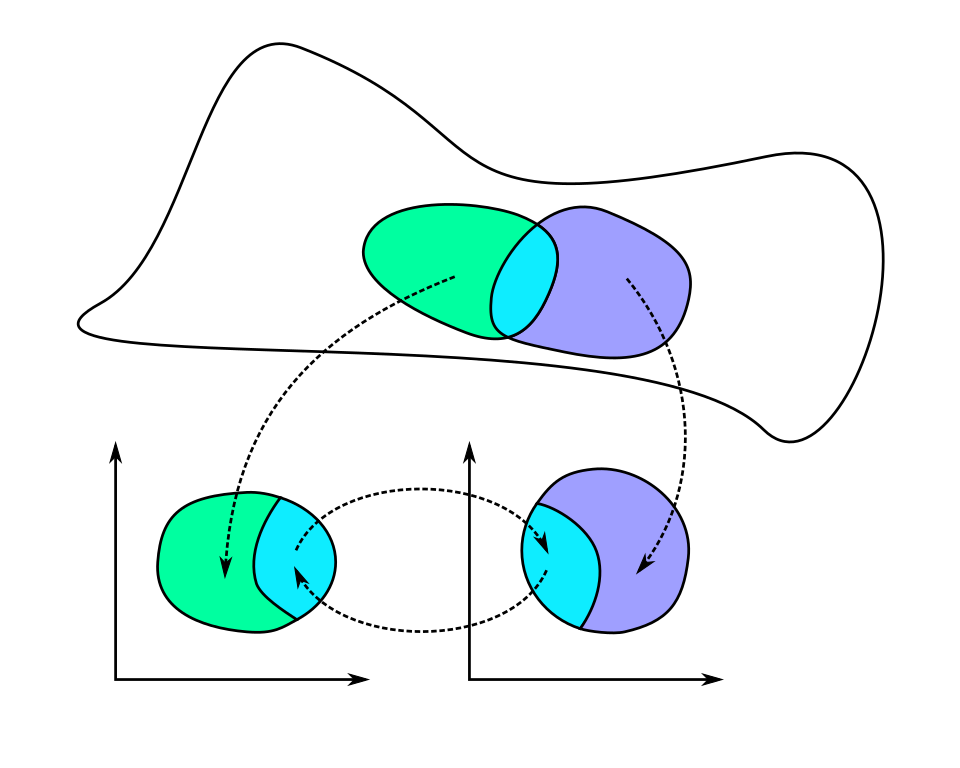
\includegraphics[scale=0.2]{Two_charts.png}
\end{figure}
\vfill
A Lie group is a continuous group with a differentiable manifold, such that group multiplication and group inverses are both differentiable.
\end{frame}

\begin{frame}
\justify
The general linear group over real numbers, $GL(n,\mathbb{R})$, is the group of all $n \times n$ invertible matrices with real entries.
\vfill
The collection of unitary matrices is a subgroup of $GL(n,\mathbb{C})$, called the unitary group $U(n)$. If we specify that the determinant is 1, then we have the special unitary group $SU(n)$.
\vfill
The collection of orthogonal matrices is a subgroup of $GL(n,\mathbb{C})$, called the orthogonal group $O(n)$. If we specify that the determinant is 1, then we have the special orthogonal group $SO(n)$.
\vfill
The exponential of a matrix is defined as
\begin{align}
\text{EXP}(X) = \sum_0^\infty \frac{X^n}{n!},
\end{align}
where $X^0$ is defined to be the identity matrix and $X^n$ is the repeated matrix product of $X$ with itself.
\end{frame}

\begin{frame}
\justify
Let $X$ and $Y$ be arbitrary $n \times n$ matrices. Then we have
\begin{enumerate}
\item $(e^X)^\dagger = e^{X^\dagger}$
\item $e^X$ is invertible and $(e^X)^{-1} = e^{-X}$
\item $e^{(\alpha + \beta)X} = e^{\alpha X} e^{\beta X}$ for all $\alpha$ and $\beta$ in $\mathbb{C}$
\item If $XY = YX$, then $e^{X+Y} = e^X e^Y = e^Y e^X$
\item If $C$ is invertible, then $e^{CXC^{-1}} = C e^X C^{-1}$
\end{enumerate}
\vfill
Particularly, if $X = CDC^{-1}$, where $D$ is a diagonal matrix with diagonal entries $\lambda_i$, then
\begin{align}
e^X = C \begin{pmatrix} e^{\lambda_1} & & 0 \\ & \ddots & \\ 0 & & e^{\lambda_n} \end{pmatrix} C^{-1}.
\end{align}
\vfill
For any matrix $X \in M_n(\mathbb{C})$, we have
\begin{align}
\text{det} (e^X) = e^{\text{Tr} (X)}.
\end{align}
\end{frame}

\begin{frame}
\justify
A function $f:\mathbb{R} \rightarrow GL(n,\mathbb{C})$ is called a one-parameter subgroup of $GL(n,\mathbb{C})$ if
\begin{enumerate}
\item $f$ is continuous,
\item $f(0)=I$,
\item $f(t+s) = f(t) f(s)$ for all $t,\,s\in\mathbb{R}$
\end{enumerate}
\vfill
The action of a one-parameter group is known as a flow, sending points along integral curves of the vector field.
\vfill
If $f$ is a one-parameter subgroup of $GL(n,\mathbb{C})$, then there exists a unique $n\times n$ complex matrix $X$ such that
\begin{align}
f(t) = e^{tX}.
\end{align}
\vfill
Let $X$ be a $n\times n$ complex matrix. Then
\begin{align}
\frac{d}{dt} e^{tX} = X e^{tX} = e^{tX} X.
\end{align}
In particular,
\begin{align}
\left. \frac{d}{dt} e^{tX} \right|_{t=0} = X.
\end{align}
\end{frame}

\begin{frame}{$SU(2)$}
\justify
$SU(2)$ is a special unitary group of dimension 2, given by unitary matrices of determinant 1. The group elements consist of
\begin{align}
SU(2) = \left\{ U = \begin{pmatrix} u_{11} & u_{12} \\ -\bar{u}_{12} & \bar{u}_{11} \end{pmatrix},\, |u_{11}|^2 + |u_{12}|^2 = 1 \right\}.
\end{align}
\vfill
Consider its one-parameter subgroup, $U(t)$.
\begin{align}
\left. \frac{d}{dt} (U(t) U^\dagger(t)) \right|_{t=0} & = \left. \frac{d}{dt} I \right|_{t=0} = 0 \nonumber \\
\left. \frac{dU}{dt} U^\dagger \right|_{t=0} + \left. U \frac{dU^\dagger}{dt} \right|_{t=0} & = 0 \nonumber \\
\left. \frac{dU}{dt} \right|_{t=0} + \left. \frac{dU^\dagger}{dt} \right|_{t=0} & = 0 \nonumber \\
X & = -X^\dagger
\end{align}
Note that $X$ is the generator of $SU(2)$.
\end{frame}

\begin{frame}
\justify
From the condition for determinant,
\begin{align}
\text{det} (e^{tX}) = e^{t \text{Tr} (X)} = 1,
\end{align}
it implies that $\text{Tr} (X) = 0$.
\vfill
Therefore, the generators of $SU(2)$ consist of traceless, anti-Hermitian matrices.
\vfill
Physicists usually absorb the anti-Hermiticity property by considering the one-parameter subgroup $f(t) = e^{itX}$. Hence, the generators of $SU(2)$ consist of traceless Hermitian matrices.
\vfill
The generators of $SU(2)$ form the Lie algebra $\mathfrak{su}(2) = \text{span} \{i\sigma_1,\, i\sigma_2,\, i\sigma_3 \}$.
\vfill
The commutation relations are
\begin{align}
[\sigma_1,\sigma_2] = 2\sigma_3,\, [\sigma_2,\sigma_3] = 2\sigma_1,\, [\sigma_3,\sigma_1] = 2\sigma_2.
\end{align}
\end{frame}

\begin{frame}{$SO(3)$}
\justify
$SO(3)$ is a special orthogonal group of dimension 3, given by orthogonal matrices of determinant 1.
\vfill
Consider its one-parameter subgroup, $O(t)$.
\begin{align}
\left. \frac{d}{dt} (O(t) O^T(t)) \right|_{t=0} & = \left. \frac{d}{dt} I \right|_{t=0} = 0 \nonumber \\
\left. \frac{dO}{dt} O^T \right|_{t=0} + \left. O \frac{dO^T}{dt} \right|_{t=0} & = 0 \nonumber \\
\left. \frac{dO}{dt} \right|_{t=0} + \left. \frac{dO^T}{dt} \right|_{t=0} & = 0 \nonumber \\
X & = -X^T
\end{align}
Note that $X$ is the generator of $SO(3)$.
\end{frame}

\begin{frame}
\justify
From the condition for determinant,
\begin{align}
\text{det} (e^{tX}) = e^{t \text{Tr} (X)} = 1,
\end{align}
it implies that $\text{Tr} (X) = 0$.
\vfill
Therefore, the Lie algebra of $SO(3)$ consist of traceless, anti-symmetric matrices,
\begin{align}
L_x = \begin{pmatrix} 0 & 0 & 0 \\ 0 & 0 & -1 \\ 0 & 1 & 0 \end{pmatrix}, L_y = \begin{pmatrix} 0 & 0 & 1 \\ 0 & 0 & 0 \\ -1 & 0 & 0 \end{pmatrix}, L_z = \begin{pmatrix} 0 & -1 & 0 \\ 1 & 0 & 0 \\ 0 & 0 & 0 \end{pmatrix}.
\end{align}
\vfill
The commutation relations are
\begin{align}
[L_x, L_y] = L_z,\, [L_y, L_z] = L_x,\, [L_z, L_x] = L_y.
\end{align}
\end{frame}

\begin{frame}{Isomorphism between $\mathfrak{so}(3)$ and $\mathfrak{su}(2)$}
\justify
The Lie algebra of $\mathfrak{so}(3)$ and $\mathfrak{su}(2)$ are isomorphic. Consider the following basis for $\mathfrak{su}(2)$,
\begin{align}
t_1 = \frac{1}{2} \begin{pmatrix} 0 & -i \\ -i & 0 \end{pmatrix},\, t_2 = \frac{1}{2} \begin{pmatrix} 0 & -1 \\ 1 & 0 \end{pmatrix},\, t_3 = \frac{1}{2} \begin{pmatrix} -i & 0 \\ 0 & i \end{pmatrix}.
\end{align}
\vfill
The commutation relations are
\begin{align}
[t_1, t_2] = t_3,\, [t_2, t_3] = t_1,\, [t_3, t_1] = t_2,
\end{align}
which is the same as the commutation relations for $\mathfrak{so}(3)$.
\vfill
However, even though the Lie algebra of $\mathfrak{su}(2)$ is isomorphic to $\mathfrak{so}(3)$, their groups are not isomorphic.
\vfill
$SU(2)$ is a double cover of $SO(3)$, meaning there is a two-to-one group homomorphism from $SU(2)$ to $SO(3)$.
\end{frame}

\begin{frame}
\justify
Recall that the one-qubit state can be written as
\begin{align*}
|\psi\rangle = \cos\left(\frac{\theta}{2}\right) |0\rangle + e^{i \phi} \sin\left(\frac{\theta}{2}\right) |1\rangle.
\end{align*}
\vfill
Its density matrix is given by
\begin{align*}
\rho & = \begin{pmatrix}
\cos^2 \left(\frac{\theta}{2}\right) & e^{-i\phi} \sin \left(\frac{\theta}{2}\right) \cos \left(\frac{\theta}{2}\right) \\ e^{i\phi} \sin \left(\frac{\theta}{2}\right) \cos \left(\frac{\theta}{2}\right) & \sin^2 \left(\frac{\theta}{2}\right)
\end{pmatrix}.
\end{align*}
\vfill
Also,
\begin{align*}
P_x = \langle\psi|X|\psi\rangle & = \sin\theta \cos\phi, \\
P_y = \langle\psi|Y|\psi\rangle & = \sin\theta \sin\phi, \\
P_z = \langle\psi|Z|\psi\rangle & = \cos\theta.
\end{align*}
\end{frame}

\begin{frame}
\justify
Writing the density matrix in terms of $\{P_x,\, P_y,\, P_z\}$, the polarization (Bloch) vectors,
\begin{align*}
\rho & = \begin{pmatrix}
\frac{\cos\theta +1}{2} & \frac{\sin\theta(\cos\phi - i \sin\phi)}{2} \\ \frac{\sin\theta (\cos\phi + i\sin\phi)}{2} & \frac{1-\cos\theta}{2}
\end{pmatrix} \nonumber \\
& = \frac{1}{2} \begin{pmatrix}
P_z + 1 & P_x - i P_y \\ P_x + iP_y & 1 - P_z
\end{pmatrix} \nonumber \\
& = \frac{1}{2} \left( I + P_x X + P_y Y + P_z Z \right) \nonumber \\
& = \frac{1}{2} \left( I + \vec{P} \cdot \vec{\sigma} \right),
\end{align*}
where
\begin{align*}
\vec{P} = \begin{pmatrix} P_x \\ P_y \\ P_z \end{pmatrix},\, \vec{\sigma} = \begin{pmatrix} X \\ Y \\ Z \end{pmatrix}.
\end{align*}
\end{frame}

\section{QMS Journal Club 13th meeting}
\begin{frame}
\vfill
\centering
\begin{beamercolorbox}[sep=8pt,center,shadow=true,rounded=true]{title}
\Large QMS Journal Club 13th meeting
\end{beamercolorbox}
\vfill
\end{frame}

\begin{frame}{Quantum algorithms}
\justify
\begin{figure}[h!]
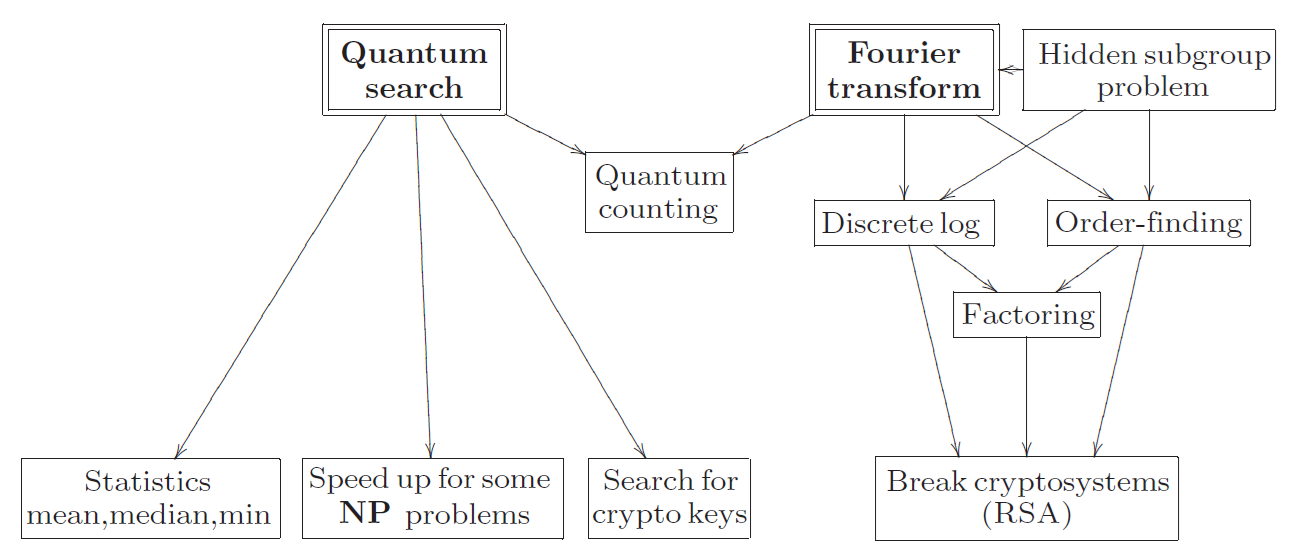
\includegraphics[scale=0.3]{Quantum_algorithms.png}
\end{figure}
\vfill
Finding good quantum algorithms is difficult because
\begin{enumerate}
\item we want our algorithm to be better than the best known classical algorithm;
\item we are much better adapted to the classical world.
\end{enumerate}
\end{frame}

\begin{frame}{Quantum gates}
\justify
The Pauli gates are
\begin{align*}
\sigma_0 = I = \begin{pmatrix} 1 & 0 \\ 0 & 1 \end{pmatrix},\,& \sigma_1 = X = \begin{pmatrix} 0 & 1 \\ 1 & 0 \end{pmatrix}, \\
\sigma_2 = Y = \begin{pmatrix} 0 & -i \\ i & 0 \end{pmatrix},\,& \sigma_3 = Z = \begin{pmatrix} 1 & 0 \\ 0 & -1 \end{pmatrix}.
\end{align*}
\vfill
In addition, we have
\begin{align*}
H & = \frac{1}{\sqrt{2}} \begin{pmatrix} 1 & 1 \\ 1 & -1 \end{pmatrix},\, S = \begin{pmatrix} 1 & 0 \\ 0 & i \end{pmatrix}, \\
T & = \begin{pmatrix} 1 & 0 \\ 0 & e^{i\frac{\pi}{4}} \end{pmatrix}.
\end{align*}
\vfill
We take note that $H=\frac{X+Z}{\sqrt{2}}$ and $S = T^2$.
\end{frame}

\begin{frame}
\justify
The Pauli matrices give rise to three useful classes of unitary matrices when they are exponentiated, i.e. the rotation operators,
\begin{align}
R_x(\theta) & = e^{-\frac{i\theta X}{2}} = \cos \frac{\theta}{2}I - i \sin \frac{\theta}{2} X = \begin{pmatrix} \cos \frac{\theta}{2} & -i \sin \frac{\theta}{2} \\ -i \sin \frac{\theta}{2} & \cos \frac{\theta}{2} \end{pmatrix}, \\
R_y(\theta) & = e^{-\frac{i\theta Y}{2}} = \cos \frac{\theta}{2}I - i \sin \frac{\theta}{2} Y = \begin{pmatrix} \cos \frac{\theta}{2} & - \sin \frac{\theta}{2} \\ \sin \frac{\theta}{2} & \cos \frac{\theta}{2} \end{pmatrix}, \\
R_z(\theta) & = e^{-\frac{i\theta Z}{2}} = \cos \frac{\theta}{2}I - i \sin \frac{\theta}{2} Z = \begin{pmatrix} e^{\frac{-i \theta}{2}} & 0 \\ 0 & e^{\frac{i \theta}{2}} \end{pmatrix}.
\end{align}
\vfill
\textbf{Exercise:} Let $x$ be a real number and $A$ a matrix such that $A^2 = I$. Show that
\begin{align}
e^{iAx} = I \cos x + i A \sin x.
\end{align}
\vfill
\textbf{Exercise:} Express Hadamard gate $H$ as a product of $R_x$ and $R_z$ rotations and $e^{i\phi}$ for some $\phi$.
\end{frame}

\begin{frame}
\justify
If $\hat{n} = (n_x,\,n_y,\,n_z)$ is a real unit vector in three dimensions, then we can generalize a rotation by $\theta$ about the $\hat{n}$ axis by
\begin{align}
R_{\hat{n}}(\theta) = e^{\frac{-i\theta \hat{n} \cdot \vec{\sigma}}{2}} = \cos \frac{\theta}{2} I - i \sin \frac{\theta}{2} (n_x X + n_y Y + n_z Z),
\end{align}
where $\vec{\sigma}$ denotes the pseudovector of Pauli matrices.
\vfill
\textbf{Exercise:} Show that $(\hat{n}\cdot\vec{\sigma})^2 = I$ and use this to verify the equation above.
\vfill
\textbf{Exercise:} Show that $XYX = -Y$ and use this to prove that $X R_y(\theta) X = R_y(-\theta)$.
\end{frame}

\begin{frame}
\justify
An arbitrary unitary operator on a single qubit can be written in many ways as a combination of rotations, together with global phase shifts on the qubit.
\vfill
\textbf{Theorem ($Z$-$Y$ decomposition):} Suppose $U$ is a unitary operation on a single qubit. Then there exist real numbers $\alpha$, $\beta$, $\gamma$, and $\delta$ such that
\begin{align}
U = e^{i \alpha} R_z(\beta) R_y(\gamma) R_z(\delta).
\end{align}
\vfill
\textbf{Corollary ($Z$-$Y$ decomposition):} Suppose $U$ is a unitary gate on a single qubit. Then there exist unitary operators $A$, $B$, $C$ on a single qubit such that $ABC = I$ and $U = e^{i \alpha} AXBXC$, where $\alpha$ is some overall phase factor.
\vfill
\textbf{Exercise:} Give $A$, $B$, $C$, and $\alpha$ for the Hadamard gate.
\vfill
\textbf{\textcolor[rgb]{1,0,0}{Exercise ($X$-$Y$ decomposition):}} Give a decomposition analogous to the $Z$-$Y$ decomposition but using $R_x$ instead of $R_z$.
\end{frame}

\begin{frame}
\justify
\textbf{Exercise:} Prove the following identities:
\begin{align}
HXH & = Z, \\
HYH & = -Y, \\
HZH & = X.
\end{align}
\vfill
\textbf{Exercise:} Use the identities above to show that $HTH = R_x (\frac{\pi}{4})$, up to a global phase.
\vfill
\textbf{\textcolor[rgb]{1,0,0}{Exercise:}} The Bloch representation gives a nice way to visualize the effect of composing two rotations. Prove that if a rotation through an angle $\beta_1$ about the axis $\hat{n}_1$ is followed by a rotation through an angle $\beta_2$ about an axis $\hat{n}_2$, then the overall rotation is through an angle $\beta_{12}$ about an axis $\hat{n}_{12}$, given by
\begin{align}
c_{12} & = c_1 c_2 - s_1 s_2 \hat{n}_1 \cdot \hat{n}_2, \\
s_{12} \hat{n}_{12} & = s_1 c_2 \hat{n}_1 + c_1 s_2 \hat{n}_2 - s_1 s_2 \hat{n}_2 \times \hat{n}_1,
\end{align}
where $c_i = \cos (\frac{\beta_i}{2})$, $s_i = \sin (\frac{\beta_i}{2})$, $c_{12} = \cos (\frac{\beta_{12}}{2})$, and $s_{12} = \sin (\frac{\beta_{12}}{2})$.
\end{frame}

\section{QMS Journal Club 14th meeting}
\begin{frame}
\vfill
\centering
\begin{beamercolorbox}[sep=8pt,center,shadow=true,rounded=true]{title}
\Large QMS Journal Club 14th meeting
\end{beamercolorbox}
\vfill
\end{frame}

\begin{frame}{Controlled operations}
\justify
A control operation is a quantum gate with two input qubits, known as the control qubit and target qubit.
\vfill
In terms of the computational basis, the action of a control-NOT gate, also known as $CNOT$, is given by $|c\rangle |t\rangle \rightarrow |c\rangle |t\oplus c\rangle$,
\begin{align}
CNOT = \begin{pmatrix} 1 & 0 & 0 & 0 \\ 0 & 1 & 0 & 0 \\ 0 & 0 & 0 & 1 \\ 0 & 0 & 1 & 0 \end{pmatrix},
\end{align}
and it is represented as
\begin{figure}
\begin{quantikz}
& \ctrl{1} & \\
& \targ{}  &
\end{quantikz}
\caption{$CNOT$ gate}
\end{figure}
\end{frame}

\begin{frame}
\justify
More generally, a control-$U$ operation is given by $|c\rangle |t\rangle \rightarrow |c\rangle U^c|t\rangle$ and represented as
\begin{figure}
\begin{quantikz}
& \ctrl{1} & \\
& \gate{U}  &
\end{quantikz}
\caption{Control-$U$ gate}
\end{figure}
\vfill
\textbf{Exercise:} Construct a $CNOT$ gate from one control-$Z$ gate, i.e. the gate whose action in the computational basis is specified by the unitary matrix
\begin{align}
CZ = \begin{pmatrix} 1 & 0 & 0 & 0 \\ 0 & 1 & 0 & 0 \\ 0 & 0 & 1 & 0 \\ 0 & 0 & 0 & -1 \end{pmatrix},
\end{align}
and two Hadamard gates.
\end{frame}

\begin{frame}
\justify
\textbf{Exercise:} Show that
\begin{figure}
\begin{quantikz}
& \ctrl{1} & \\
& \gate{Z}  &
\end{quantikz} = \begin{quantikz}
& \gate{Z} & \\
& \ctrl{-1}  &
\end{quantikz}
\end{figure}
\vfill
\textbf{Exercise:} Show that the $CNOT$ gate is a simple permutation on a density matrix $\rho$.
\end{frame}

\begin{frame}
\justify
\textbf{Exercise:} The roles of ``control" and ``target" qubits are arbitrary, i.e. they depend on the basis they are operating in. In computational basis, the state of the control qubit is not changed. However, if we work in a different basis, the control qubit does change. Show that
\begin{figure}
\begin{quantikz}
& \gate{H} & \ctrl{1} & \gate{H} & \\
& \gate{H} & \targ{}  & \gate{H} &
\end{quantikz} = \begin{quantikz}
& \targ{} & \\
& \ctrl{-1}  &
\end{quantikz}
\end{figure}
Hence, show that
\begin{align*}
|++\rangle & \rightarrow |++\rangle \\
|-+\rangle & \rightarrow |-+\rangle \\
|+-\rangle & \rightarrow |--\rangle \\
|--\rangle & \rightarrow |+-\rangle
\end{align*}
\end{frame}

\begin{frame}
\justify
In order to implement control-$U$ operation for arbitrary single qubit using only single qubit operations and $CNOT$ gate, one can make use of the decomposition
\begin{align}
U = e^{i\alpha} AXBXC,
\end{align}
where $ABC = I$.
\vfill
The first step is to apply the phase shift $e^{i\alpha}$ that produces the effect
\begin{align*}
|00\rangle & \rightarrow |00\rangle \\
|01\rangle & \rightarrow |01\rangle \\
|10\rangle & \rightarrow e^{i\alpha} |10\rangle \\
|11\rangle & \rightarrow e^{i\alpha} |11\rangle
\end{align*}
\end{frame}

\begin{frame}
\justify
One may verify that the following is equivalent,
\begin{figure}
\begin{quantikz}
& \ctrl{1} & \\
& \gate{\begin{pmatrix} e^{i\alpha} & 0 \\ 0 & e^{i\alpha} \end{pmatrix}} &
\end{quantikz} = \begin{quantikz}
& \gate{\begin{pmatrix} 1 & 0 \\ 0 & e^{i\alpha} \end{pmatrix}} & \\
& &
\end{quantikz}
\end{figure}
\vfill
Hence, a control-$U$ gate can be implemented as
\begin{figure}
\begin{quantikz}
& & \ctrl{1} & & \ctrl{1} & \gate{\begin{pmatrix} 1 & 0 \\ 0 & e^{i\alpha} \end{pmatrix}} & \\
& \gate{C} & \targ{} & \gate{B} & \targ{} & \gate{A} &
\end{quantikz}
\end{figure}
\end{frame}

\end{document}